\documentclass[aspectratio=169,11pt]{beamer}
\geometry{paperwidth=19.2cm,paperheight=10.8cm}
\usepackage{fontspec}
\usepackage{booktabs}
\usepackage{array}
\usepackage{etoolbox}
\usepackage{tikz}
\usetikzlibrary{positioning,arrows.meta,shapes.geometric,calc,fit,backgrounds}

% ink is the indigo of the IIT Kharagpur logo (img/iitkgp_logo.pdf); the rest are tints of it plus a saffron accent
\definecolor{bg}{HTML}{F6F5FB}
\definecolor{ink}{HTML}{291973}
\definecolor{iris}{HTML}{5B4FB0}
\definecolor{saffron}{HTML}{B45309}
\definecolor{gold}{HTML}{F2C14E}
\definecolor{haze}{HTML}{EEECF7}
\definecolor{muted}{HTML}{6C6889}
\definecolor{rule}{HTML}{D5D1E8}

\setbeamercolor{background canvas}{bg=white}
\setbeamercolor{normal text}{fg=ink}
\setbeamercolor{structure}{fg=iris}
\setbeamertemplate{navigation symbols}{}
\setbeamertemplate{itemize item}{\textcolor{saffron}{\rule[.25ex]{.9ex}{.9ex}}}
\setbeamercolor{frametitle}{fg=white,bg=ink}
\setbeamercolor{footline}{fg=white,bg=ink}
\setbeamertemplate{frametitle}{%
  \nointerlineskip
  % baseline 6.7 mm down a 10.5 mm bar puts the capitals on the same centre line as the logo and the tag
  \begin{beamercolorbox}[wd=\paperwidth,ht=6.7mm,dp=3.8mm,leftskip=6mm,rightskip=16mm]{frametitle}%
    \large\bfseries\insertframetitle
  \end{beamercolorbox}%
  \begin{tikzpicture}[remember picture,overlay]
    \fill[gold] ([yshift=-10.5mm]current page.north west) rectangle ([yshift=-11.1mm]current page.north east);
    \node[anchor=east,inner sep=0] at ([xshift=-5mm,yshift=-5.25mm]current page.north east) {
\includegraphics[height=8mm]{img/iitkgp_logo_white}};
    \ifx\badge\relax\else\node[anchor=east,fill=gold,text=ink,font=\tiny\bfseries,rounded corners=2pt,inner sep=2.5pt] at ([xshift=-16mm,yshift=-5.25mm]current page.north east) {\badge};\fi
  \end{tikzpicture}\vspace{2.5mm}}
% frames wrapped in {\newsince ...} get the tag; everything else leaves \badge at \relax
\let\badge\relax
\newcommand{\newsince}{\def\badge{NEW SINCE MID-TERM}}
\setbeamertemplate{footline}{%
  \begin{beamercolorbox}[wd=\paperwidth,ht=3.2mm,dp=1.6mm,leftskip=6mm,rightskip=6mm]{footline}%
    \scriptsize Indian Institute of Technology Kharagpur \quad PhysioBase\hfill{\color{gold}\insertframenumber\,/\,\inserttotalframenumber}
  \end{beamercolorbox}}
\setbeamersize{text margin left=6mm,text margin right=6mm}

\tikzset{
  card/.style={rounded corners=3pt,fill=haze,draw=rule,line width=.4pt,align=left},
  step/.style={rounded corners=3pt,fill=white,draw=rule,line width=.5pt,align=left,
    text width=#1,inner sep=4pt,font=\scriptsize},
  step/.default=2.55cm,
  flowarrow/.style={-{Stealth[length=2.2mm]},line width=.9pt,iris},
  num/.style={circle,fill=saffron,text=white,font=\scriptsize\bfseries,inner sep=1.5pt,minimum size=4.5mm},
}
\newcommand{\bignum}[1]{{\color{saffron}\fontsize{22}{24}\selectfont #1}}
\newcommand{\capt}[1]{{\color{iris}\scriptsize\bfseries #1}}
\newcommand{\sw}[1]{\tikz[baseline=-.6ex]\fill[#1] (0,0) circle (2.2pt);}

\AtBeginDocument{\hyphenpenalty=10000 \exhyphenpenalty=10000}
\makeatletter
\newcommand{\ra}{\ifdefequal{\f@series}{\bfdefault}{{\boldmath$\rightarrow$}}{$\rightarrow$}}
\makeatother
% open items stay visible on the slide until they are answered
\newcommand{\phline}[1]{{\color{saffron}\bfseries #1}}
\newsavebox\herobox

\begin{document}
\sbox\herobox{% title and thanks hero: what a person writes, what the wristband adds, what the model answers.
% set once into \herobox, so both slides draw the same picture
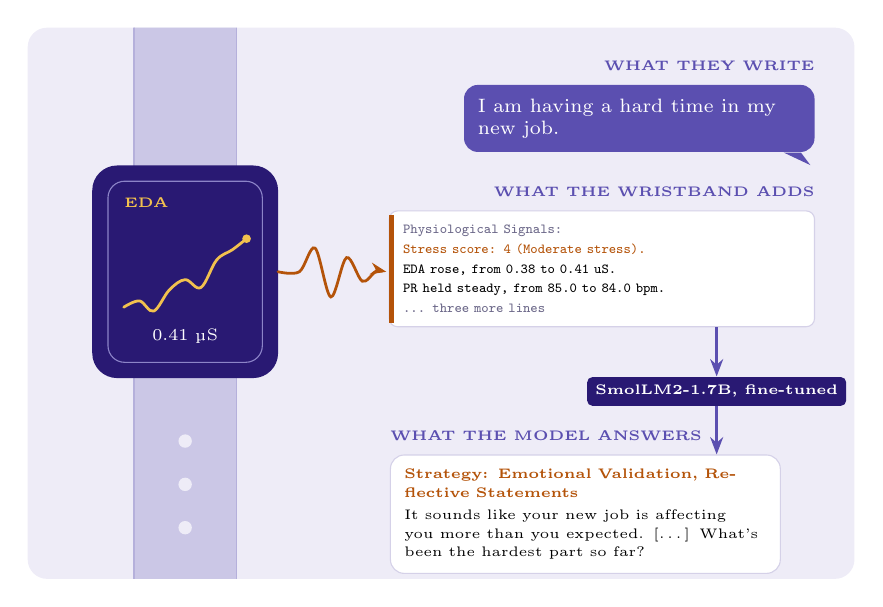
\begin{tikzpicture}[x=1cm,y=1cm,
    lbl/.style={inner sep=0,font=\fontsize{5.5}{6.5}\selectfont\bfseries,text=iris}]
  \fill[haze,rounded corners=7pt] (0,0) rectangle (10.5,-7);
  \begin{scope}
    \clip[rounded corners=7pt] (0,0) rectangle (10.5,-7);
    \fill[iris!32] (1.35,.1) rectangle (2.65,-7.1);
    \draw[iris!45,line width=.4pt] (1.35,.1) -- (1.35,-7.1) (2.65,.1) -- (2.65,-7.1);
    \foreach \y in {-5.25,-5.8,-6.35}{\fill[haze] (2,\y) circle (.085);}
  \end{scope}

  \fill[ink,rounded corners=9pt] (.82,-1.75) rectangle (3.18,-4.45);
  \draw[iris!70,line width=.4pt,rounded corners=6pt] (1.02,-1.95) rectangle (2.98,-4.25);
  \node[anchor=north west,inner sep=0,text=gold,font=\fontsize{5.5}{6.5}\selectfont\bfseries] at (1.22,-2.15) {EDA};
  \draw[gold,line width=1pt,line cap=round,line join=round] plot[smooth,tension=.6] coordinates
    {(1.22,-3.55) (1.42,-3.47) (1.6,-3.6) (1.8,-3.33) (2,-3.2) (2.2,-3.3) (2.4,-2.95) (2.6,-2.82) (2.78,-2.68)};
  \fill[gold] (2.78,-2.68) circle (.055);
  \node[inner sep=0,text=white,font=\fontsize{6}{7}\selectfont] at (2,-3.92) {0.41 µS};

  \node[lbl,anchor=north east] at (10,-.42) {WHAT THEY WRITE};
  \node[anchor=north east,fill=iris,text=white,rounded corners=5pt,text width=4.1cm,inner sep=5pt,
    font=\scriptsize,align=left] (msg) at (10,-.72) {I am having a hard time in my new job.};
  \fill[iris] ([xshift=-4mm]msg.south east) -- ++(.22,0) -- ++(.12,-.16) -- cycle;

  \node[lbl,anchor=north east] at (10,-2.02) {WHAT THE WRISTBAND ADDS};
  \node[anchor=north east,fill=white,draw=rule,line width=.4pt,rounded corners=3pt,text width=5.05cm,
    inner sep=5pt,font=\ttfamily\fontsize{5.5}{7.2}\selectfont,align=left] (sum) at (10,-2.32) {%
    {\color{muted}Physiological Signals:}\\
    {\color{saffron}\bfseries Stress score: 4 (Moderate stress).}\\
    EDA rose, from 0.38 to 0.41 uS.\\
    PR held steady, from 85.0 to 84.0 bpm.\\
    {\color{muted}... three more lines}};
  \fill[saffron] (sum.north west) ++(0,-.06) rectangle ([xshift=.07cm,yshift=.06cm]sum.south west);

  \draw[saffron,line width=1pt,line cap=round,-{Stealth[length=2mm]}] plot[smooth,tension=.55] coordinates
    {(3.18,-3.1) (3.45,-3.1) (3.65,-2.8) (3.85,-3.42) (4.05,-2.92) (4.25,-3.22) (4.42,-3.1) ($(sum.west |- 0,-3.1)+(-.03,0)$)};

  \node[fill=ink,text=white,rounded corners=2pt,inner sep=3pt,font=\fontsize{5.5}{6.5}\selectfont\bfseries]
    (llm) at (8.75,-4.62) {SmolLM2-1.7B, fine-tuned};
  \draw[flowarrow] (sum.south -| llm) -- (llm);

  \node[lbl,anchor=north west] at (4.6,-5.12) {WHAT THE MODEL ANSWERS};
  \node[anchor=north west,fill=white,draw=rule,line width=.4pt,rounded corners=5pt,text width=4.6cm,
    inner sep=5pt,minimum height=1.08cm,align=left,font=\fontsize{5.5}{6.8}\selectfont] (ans) at (4.6,-5.42) {%
    {\color{saffron}\bfseries Strategy: Emotional Validation, Reflective Statements}\\[.4mm]
    It sounds like your new job is affecting you more than you expected. [\dots] What's been the hardest part so far?};
  \draw[flowarrow] (llm) -- (llm |- ans.north);
\end{tikzpicture}%
}

% ---------------------------------------------------------------- title
{\setbeamertemplate{footline}{}
\begin{frame}[plain]
\begin{tikzpicture}[remember picture,overlay]
  \fill[ink] (current page.north west) rectangle ([xshift=6.9cm]current page.south west);
  \fill[gold] ([xshift=6.9cm]current page.north west) rectangle ([xshift=7.05cm]current page.south west);
  \node[anchor=north west,inner sep=0] (logo) at ([xshift=5mm,yshift=-6mm]current page.north west) {
\includegraphics[height=1.6cm]{img/iitkgp_logo_white}};
  \node[anchor=west,text=white,font=\footnotesize\bfseries,align=left] at ([xshift=3mm]logo.east) {Indian Institute of\\Technology Kharagpur};
  \node[anchor=north west,text width=5.8cm,text=white,align=left,inner sep=0] at ([xshift=5.5mm,yshift=-28mm]current page.north west) {%
    {\color{gold}\fontsize{6.5}{8}\selectfont\bfseries FINAL EVALUATION\par}\vspace{3.5mm}
    {\fontsize{15}{18.5}\selectfont\bfseries PhysioBase:\\Physiology-Aware\\Conversational Support\par}\vspace{3mm}
    {\small An emotional support model that reads a wristband's signal summary before it answers\par}\vspace{4mm}
    {\footnotesize\begin{tabular}{@{}l@{}}Ashutosh Sharma\\B. Siddaarth\\Krishna Chaitanya\\Nithish Kumar Mahesepu\end{tabular}\par}\vspace{2mm}
    {\scriptsize Mentor: Sudipa Garain\par}\vspace{4mm}
    {\color{gold}\scriptsize November 2026\par}};
  \node[anchor=center,inner sep=0] at ([xshift=13.125cm]current page.west) {\usebox\herobox};
\end{tikzpicture}
\end{frame}}

% ---------------------------------------------------------------- objective
\begin{frame}{Does a wristband's signal summary change how a support model answers?}{BACKGROUND AND OBJECTIVES}
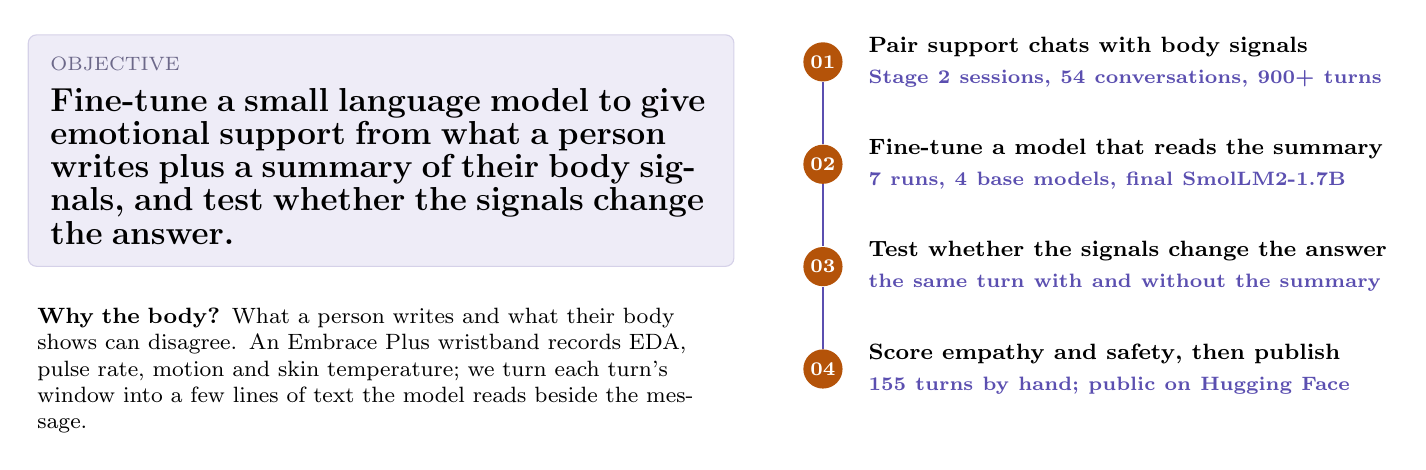
\begin{tikzpicture}
  \node[card,text width=8.4cm,inner sep=8pt,anchor=north west] (q) at (0,0) {%
    {\color{muted}\scriptsize OBJECTIVE}\\[1mm]
    {\large\bfseries Fine-tune a small language model to give emotional support from what a person writes plus a summary of their body signals, and test whether the signals change the answer.}};
  \node[anchor=north west,text width=8.4cm,font=\footnotesize] (why) at ([yshift=-4mm]q.south west) {%
    \textbf{Why the body?} What a person writes and what their body shows can disagree. An Embrace Plus wristband records EDA, pulse rate, motion and skin temperature; we turn each turn's window into a few lines of text the model reads beside the message.};
  \foreach \i/\t/\s in {1/Pair support chats with body signals/Stage 2 sessions{,} 54 conversations{,} 900+ turns,2/Fine-tune a model that reads the summary/7 runs{,} 4 base models{,} final SmolLM2-1.7B,3/Test whether the signals change the answer/the same turn with and without the summary,4/Score empathy and safety{,} then publish/155 turns by hand; public on Hugging Face}{
    \node[num] (n\i) at (10.1,-.35-1.3*\i+1.3) {0\i};
    \node[anchor=west,text width=6.6cm,align=left] at ($(n\i.east)+(.2,0)$) {\footnotesize\bfseries\t\\[-.3mm]\capt{\s}};
  }
  \draw[iris,line width=.8pt] (n1) -- (n2) -- (n3) -- (n4);
\end{tikzpicture}
\vfill
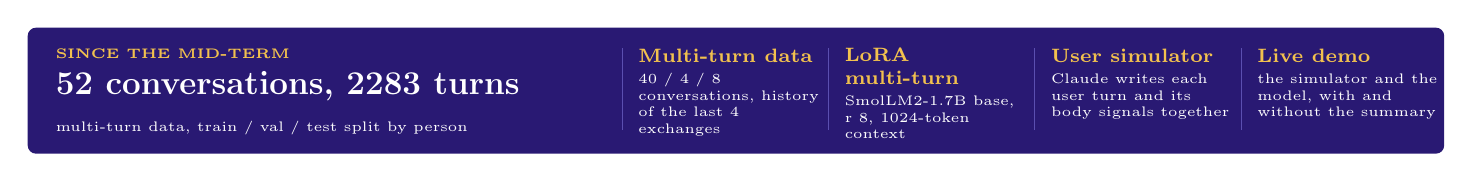
\begin{tikzpicture}
  \fill[ink,rounded corners=3pt] (0,0) rectangle (17.99,1.6);
  \node[anchor=north west,inner sep=0,text=gold,font=\tiny\bfseries] at (.35,1.34) {SINCE THE MID-TERM};
  \node[anchor=north west,inner sep=0,text=white] at (.35,1.05) {\fontsize{13}{15}\selectfont\bfseries 52 conversations, 2283 turns};
  \node[anchor=north west,inner sep=0,text=white,font=\tiny] at (.35,.42) {multi-turn data, train / val / test split by person};
  \foreach \t/\d [count=\i] in {Multi-turn data/{40 / 4 / 8 conversations, history of the last 4 exchanges},LoRA multi-turn/SmolLM2-1.7B base{,} r~8{,} 1024-token context,User simulator/Claude writes each user turn and its body signals together,Live demo/the simulator and the model{,} with and without the summary}{
    \draw[iris,line width=.4pt] (7.55+2.62*\i-2.62,.3) -- ++(0,1.04);
    \node[anchor=north west,inner sep=0,text width=2.3cm,align=flush left] at (7.75+2.62*\i-2.62,1.34) {{\color{gold}\scriptsize\bfseries\t\par}\vspace{.6mm}{\color{white}\tiny\d\par}};
  }
\end{tikzpicture}
\end{frame}

% ---------------------------------------------------------------- pipeline
\begin{frame}{From a wristband to a scored reply}{METHOD \textperiodcentered\ END-TO-END PIPELINE}
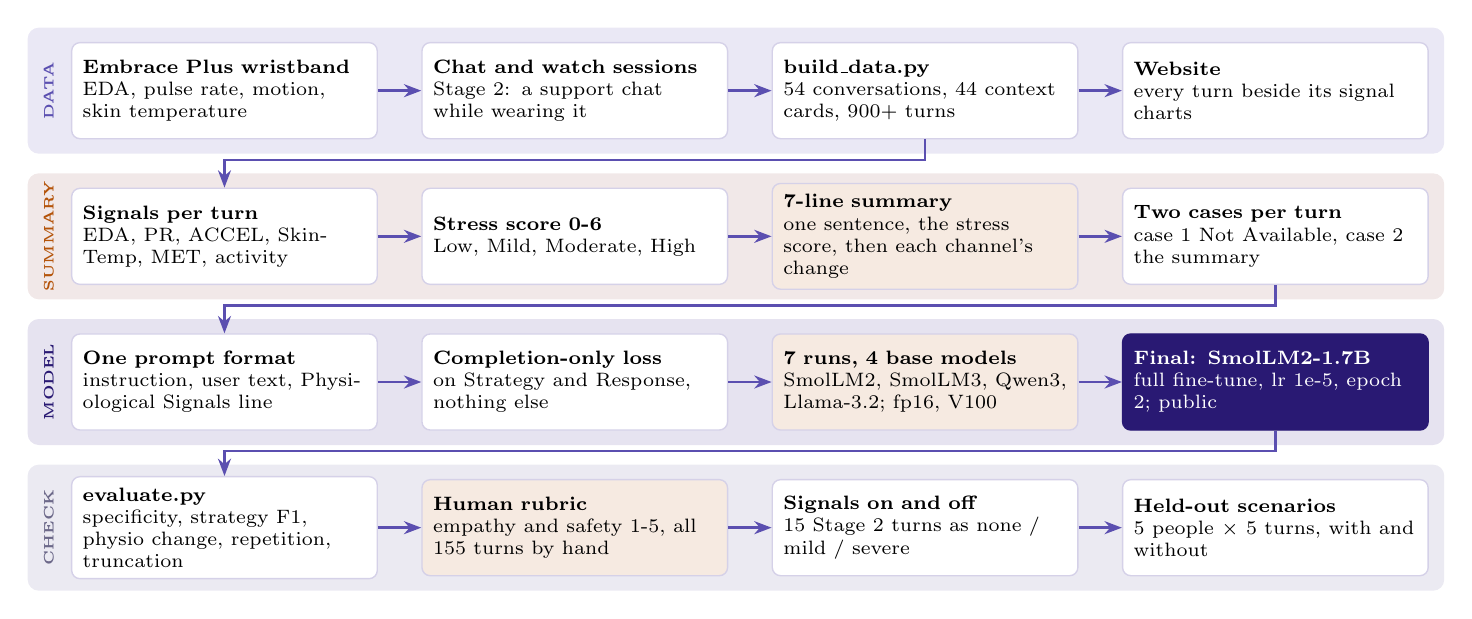
\begin{tikzpicture}[node distance=5.5mm,step/.append style={text width=3.6cm,minimum height=1.22cm}]
  \foreach \y/\c/\t in {0/iris/DATA,-1.85/saffron/SUMMARY,-3.7/ink/MODEL,-5.55/muted/CHECK}{
    \fill[\c!8!bg,rounded corners=4pt] (0,\y+.8) rectangle (17.99,\y-.8);
    \node[rotate=90,font=\tiny\bfseries,text=\c] at (.27,\y) {\t};
  }
  \node[step,anchor=west] (d1) at (.55,0) {\textbf{Embrace Plus wristband}\\EDA, pulse rate, motion, skin temperature};
  \node[step,right=of d1] (d2) {\textbf{Chat and watch sessions}\\Stage 2: a support chat while wearing it};
  \node[step,right=of d2] (d3) {\textbf{build\_data.py}\\54 conversations, 44 context cards, 900+ turns};
  \node[step,right=of d3] (d4) {\textbf{Website}\\every turn beside its signal charts};
  \node[step,anchor=west] (p1) at (.55,-1.85) {\textbf{Signals per turn}\\EDA, PR, ACCEL, SkinTemp, MET, activity};
  \node[step,right=of p1] (p2) {\textbf{Stress score 0-6}\\Low, Mild, Moderate, High};
  \node[step,right=of p2,fill=saffron!12] (p3) {\textbf{7-line summary}\\one sentence, the stress score, then each channel's change};
  \node[step,right=of p3] (p4) {\textbf{Two cases per turn}\\case 1 Not Available, case 2 the summary};
  \node[step,anchor=west] (m1) at (.55,-3.7) {\textbf{One prompt format}\\instruction, user text, Physiological Signals line};
  \node[step,right=of m1] (m2) {\textbf{Completion-only loss}\\on Strategy and Response, nothing else};
  \node[step,right=of m2,fill=saffron!12] (m3) {\textbf{7 runs, 4 base models}\\SmolLM2, SmolLM3, Qwen3, Llama-3.2; fp16, V100};
  \node[step,right=of m3,fill=ink,text=white,draw=ink] (m4) {\textbf{Final: SmolLM2-1.7B}\\full fine-tune, lr 1e-5, epoch 2; public};
  \node[step,anchor=west] (k1) at (.55,-5.55) {\textbf{evaluate.py}\\specificity, strategy F1, physio change, repetition, truncation};
  \node[step,right=of k1,fill=saffron!12] (k2) {\textbf{Human rubric}\\empathy and safety 1-5, all 155 turns by hand};
  \node[step,right=of k2] (k3) {\textbf{Signals on and off}\\15 Stage 2 turns as none / mild / severe};
  \node[step,right=of k3] (k4) {\textbf{Held-out scenarios}\\5 people $\times$ 5 turns, with and without};
  \foreach \a/\b in {d1/d2,d2/d3,d3/d4,p1/p2,p2/p3,p3/p4,m1/m2,m2/m3,m3/m4,k1/k2,k2/k3,k3/k4}{\draw[flowarrow] (\a) -- (\b);}
  \draw[flowarrow] (d3.south) -- ++(0,-.26) -| (p1.north);
  \draw[flowarrow] (p4.south) -- ++(0,-.26) -| (m1.north);
  \draw[flowarrow] (m4.south) -- ++(0,-.26) -| (k1.north);
\end{tikzpicture}
\end{frame}

% ---------------------------------------------------------------- one turn
\begin{frame}{One turn, twice: without and with the body}{DATA \textperiodcentered\ WHAT THE MODEL SEES}
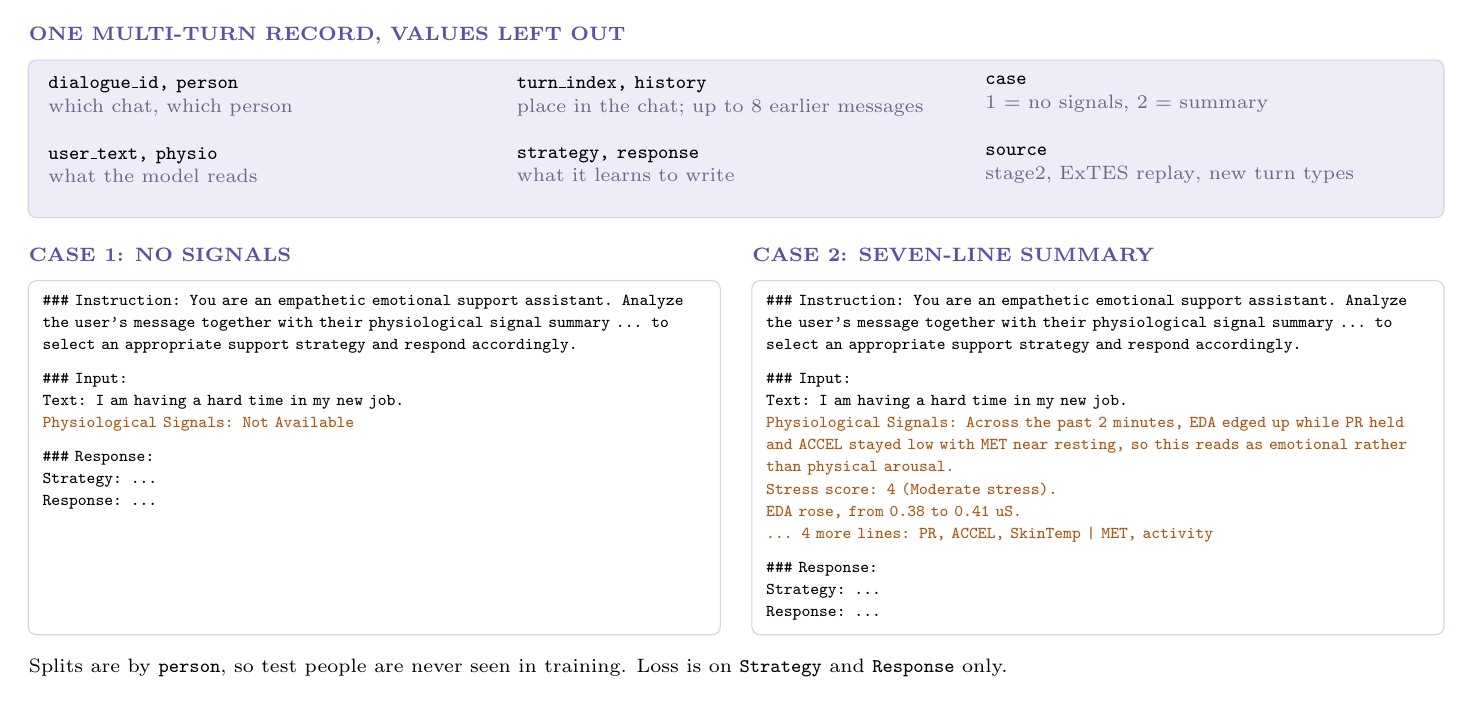
\begin{tikzpicture}
  \node[anchor=north west,inner sep=0] at (0,0) {\capt{ONE MULTI-TURN RECORD, VALUES LEFT OUT}};
  \fill[haze,draw=rule,line width=.4pt,rounded corners=3pt] (0,-.42) rectangle (17.98,-2.42);
  \foreach \x/\y/\k/\m in {
    .25/-.62/{dialogue\_id, person}/which chat{,} which person,
    6.2/-.62/{turn\_index, history}/place in the chat; up to 8 earlier messages,
    12.15/-.62/case/1 = no signals{,} 2 = summary,
    .25/-1.52/{user\_text, physio}/what the model reads,
    6.2/-1.52/{strategy, response}/what it learns to write,
    12.15/-1.52/source/stage2{,} ExTES replay{,} new turn types}{
    \node[anchor=north west,inner sep=0,text width=5.6cm,font=\scriptsize,align=left] at (\x,\y) {\texttt{\k}\\[.2mm]{\color{muted}\m}};
  }
  \foreach \x/\c/\p [count=\i] in {0/CASE 1: NO SIGNALS/{Physiological Signals: Not Available},9.19/CASE 2: SEVEN-LINE SUMMARY/{Physiological Signals: Across the past 2 minutes, EDA edged up while PR held and ACCEL stayed low with MET near resting, so this reads as emotional rather than physical arousal.\\Stress score: 4 (Moderate stress).\\EDA rose, from 0.38 to 0.41 uS.\\... 4 more lines: PR, ACCEL, SkinTemp | MET, activity}}{
    \node[anchor=north west,inner sep=0] at (\x,-2.8) {\capt{\c}};
    \node[anchor=north west,text width=8.43cm,inner sep=5pt,font=\fontsize{6.5}{8}\selectfont\ttfamily,align=left] (case\i) at (\x,-3.22) {%
      \#\#\# Instruction: You are an empathetic emotional support assistant. Analyze the user's message together with their physiological signal summary ... to select an appropriate support strategy and respond accordingly.\\[1.5mm]
      \#\#\# Input:\\
      Text: I am having a hard time in my new job.\\
      \phline{\p}\\[1.5mm]
      \#\#\# Response:\\
      Strategy: ...\\
      Response: ...};
  }
  % both prompt boxes as tall as the longer one
  \begin{pgfonlayer}{background}
    \path[fill=white,draw=rule,line width=.4pt,rounded corners=3pt] let \p1=(case1.south), \p2=(case2.south), \n1={min(\y1,\y2)} in
      (0,-3.22) rectangle (8.79,\n1) (9.19,-3.22) rectangle (17.98,\n1);
  \end{pgfonlayer}
  \path let \p1=(case1.south), \p2=(case2.south), \n1={min(\y1,\y2)} in
    node[anchor=north west,inner sep=0,font=\scriptsize] at (0,\n1-3mm) {Splits are by \texttt{person}, so test people are never seen in training. Loss is on \texttt{Strategy} and \texttt{Response} only.};
\end{tikzpicture}
\end{frame}

% ---------------------------------------------------------------- model selection
\begin{frame}{The lowest validation loss was not the best model}{MODEL SELECTION}
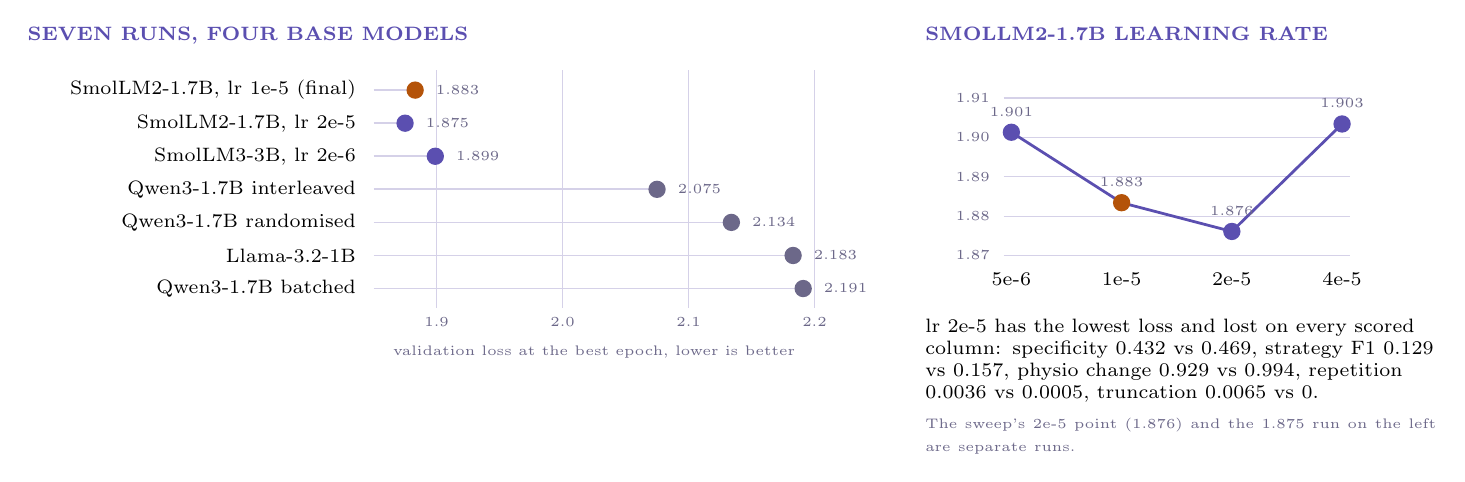
\begin{tikzpicture}
  \node[anchor=north west,inner sep=0] at (0,0) {\capt{SEVEN RUNS, FOUR BASE MODELS}};
  \begin{scope}[shift={(4.4,-.8)}]\draw[rule] (0.800,0.25) -- (0.800,-2.770);
\node[font=\tiny,text=muted,anchor=north] at (0.800,-2.770) {1.9};
\draw[rule] (2.400,0.25) -- (2.400,-2.770);
\node[font=\tiny,text=muted,anchor=north] at (2.400,-2.770) {2.0};
\draw[rule] (4.000,0.25) -- (4.000,-2.770);
\node[font=\tiny,text=muted,anchor=north] at (4.000,-2.770) {2.1};
\draw[rule] (5.600,0.25) -- (5.600,-2.770);
\node[font=\tiny,text=muted,anchor=north] at (5.600,-2.770) {2.2};
\draw[rule,line width=.6pt] (0,0.000) -- (0.528,0.000);
\fill[saffron] (0.528,0.000) circle (1.1mm);
\node[anchor=east,font=\scriptsize] at (-0.1,0.000) {SmolLM2-1.7B, lr 1e-5 (final)};
\node[anchor=west,font=\tiny,text=muted] at (0.668,0.000) {1.883};
\draw[rule,line width=.6pt] (0,-0.420) -- (0.400,-0.420);
\fill[iris] (0.400,-0.420) circle (1.1mm);
\node[anchor=east,font=\scriptsize] at (-0.1,-0.420) {SmolLM2-1.7B, lr 2e-5};
\node[anchor=west,font=\tiny,text=muted] at (0.540,-0.420) {1.875};
\draw[rule,line width=.6pt] (0,-0.840) -- (0.784,-0.840);
\fill[iris] (0.784,-0.840) circle (1.1mm);
\node[anchor=east,font=\scriptsize] at (-0.1,-0.840) {SmolLM3-3B, lr 2e-6};
\node[anchor=west,font=\tiny,text=muted] at (0.924,-0.840) {1.899};
\draw[rule,line width=.6pt] (0,-1.260) -- (3.600,-1.260);
\fill[muted] (3.600,-1.260) circle (1.1mm);
\node[anchor=east,font=\scriptsize] at (-0.1,-1.260) {Qwen3-1.7B interleaved};
\node[anchor=west,font=\tiny,text=muted] at (3.740,-1.260) {2.075};
\draw[rule,line width=.6pt] (0,-1.680) -- (4.544,-1.680);
\fill[muted] (4.544,-1.680) circle (1.1mm);
\node[anchor=east,font=\scriptsize] at (-0.1,-1.680) {Qwen3-1.7B randomised};
\node[anchor=west,font=\tiny,text=muted] at (4.684,-1.680) {2.134};
\draw[rule,line width=.6pt] (0,-2.100) -- (5.328,-2.100);
\fill[muted] (5.328,-2.100) circle (1.1mm);
\node[anchor=east,font=\scriptsize] at (-0.1,-2.100) {Llama-3.2-1B};
\node[anchor=west,font=\tiny,text=muted] at (5.468,-2.100) {2.183};
\draw[rule,line width=.6pt] (0,-2.520) -- (5.456,-2.520);
\fill[muted] (5.456,-2.520) circle (1.1mm);
\node[anchor=east,font=\scriptsize] at (-0.1,-2.520) {Qwen3-1.7B batched};
\node[anchor=west,font=\tiny,text=muted] at (5.596,-2.520) {2.191};
\node[anchor=north,font=\tiny,text=muted] at (2.800,-3.120) {validation loss at the best epoch, lower is better};
\end{scope}
  \node[anchor=north west,inner sep=0] at (11.4,0) {\capt{SMOLLM2-1.7B LEARNING RATE}};
  \begin{scope}[shift={(12.5,-2.9)}]\draw[rule] (-0.1,0.000) -- (4.300,0.000); \node[anchor=east,font=\tiny,text=muted] at (-0.15,0.000) {1.87};
\draw[rule] (-0.1,0.500) -- (4.300,0.500); \node[anchor=east,font=\tiny,text=muted] at (-0.15,0.500) {1.88};
\draw[rule] (-0.1,1.000) -- (4.300,1.000); \node[anchor=east,font=\tiny,text=muted] at (-0.15,1.000) {1.89};
\draw[rule] (-0.1,1.500) -- (4.300,1.500); \node[anchor=east,font=\tiny,text=muted] at (-0.15,1.500) {1.90};
\draw[rule] (-0.1,2.000) -- (4.300,2.000); \node[anchor=east,font=\tiny,text=muted] at (-0.15,2.000) {1.91};
\draw[iris,line width=1pt] (0.000,1.565) -- (1.400,0.670) -- (2.800,0.305) -- (4.200,1.670);
\fill[iris] (0.000,1.565) circle (1.1mm);
\node[anchor=south,font=\tiny,text=muted] at (0.000,1.645) {1.901};
\node[anchor=north,font=\scriptsize] at (0.000,-0.1) {5e-6};
\fill[saffron] (1.400,0.670) circle (1.1mm);
\node[anchor=south,font=\tiny,text=muted] at (1.400,0.750) {1.883};
\node[anchor=north,font=\scriptsize] at (1.400,-0.1) {1e-5};
\fill[iris] (2.800,0.305) circle (1.1mm);
\node[anchor=south,font=\tiny,text=muted] at (2.800,0.385) {1.876};
\node[anchor=north,font=\scriptsize] at (2.800,-0.1) {2e-5};
\fill[iris] (4.200,1.670) circle (1.1mm);
\node[anchor=south,font=\tiny,text=muted] at (4.200,1.750) {1.903};
\node[anchor=north,font=\scriptsize] at (4.200,-0.1) {4e-5};
\end{scope}
  \node[anchor=north west,text width=6.5cm,font=\scriptsize,inner sep=0] at (11.4,-3.7) {%
    lr 2e-5 has the lowest loss and lost on every scored column: specificity 0.432 vs 0.469, strategy F1 0.129 vs 0.157, physio change 0.929 vs 0.994, repetition 0.0036 vs 0.0005, truncation 0.0065 vs 0.\\[1mm]
    {\color{muted}\tiny The sweep's 2e-5 point (1.876) and the 1.875 run on the left are separate runs.}};
\end{tikzpicture}
\vfill
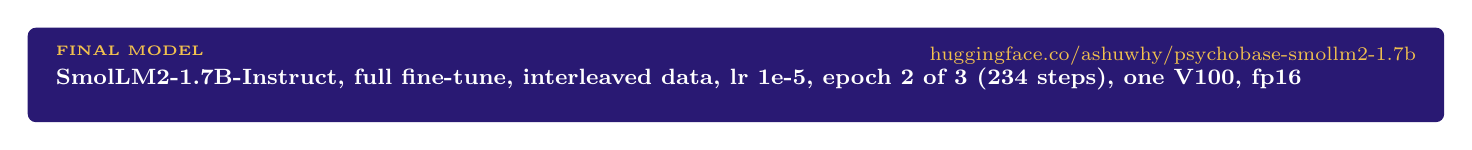
\begin{tikzpicture}
  \fill[ink,rounded corners=3pt] (0,0) rectangle (17.99,1.2);
  \node[anchor=north west,inner sep=0,text=gold,font=\tiny\bfseries] at (.35,.98) {FINAL MODEL};
  \node[anchor=north west,inner sep=0,text=white,font=\footnotesize\bfseries] at (.35,.7) {SmolLM2-1.7B-Instruct, full fine-tune, interleaved data, lr 1e-5, epoch 2 of 3 (234 steps), one V100, fp16};
  \node[anchor=north east,inner sep=0,text=gold,font=\scriptsize] at (17.64,.98) {huggingface.co/ashuwhy/psychobase-smollm2-1.7b};
\end{tikzpicture}
\end{frame}

% ---------------------------------------------------------------- bugs and F1
\begin{frame}{Four bugs we caught, and a strategy F1 below the majority guess}{TRAINING \textperiodcentered\ WHAT WENT WRONG}
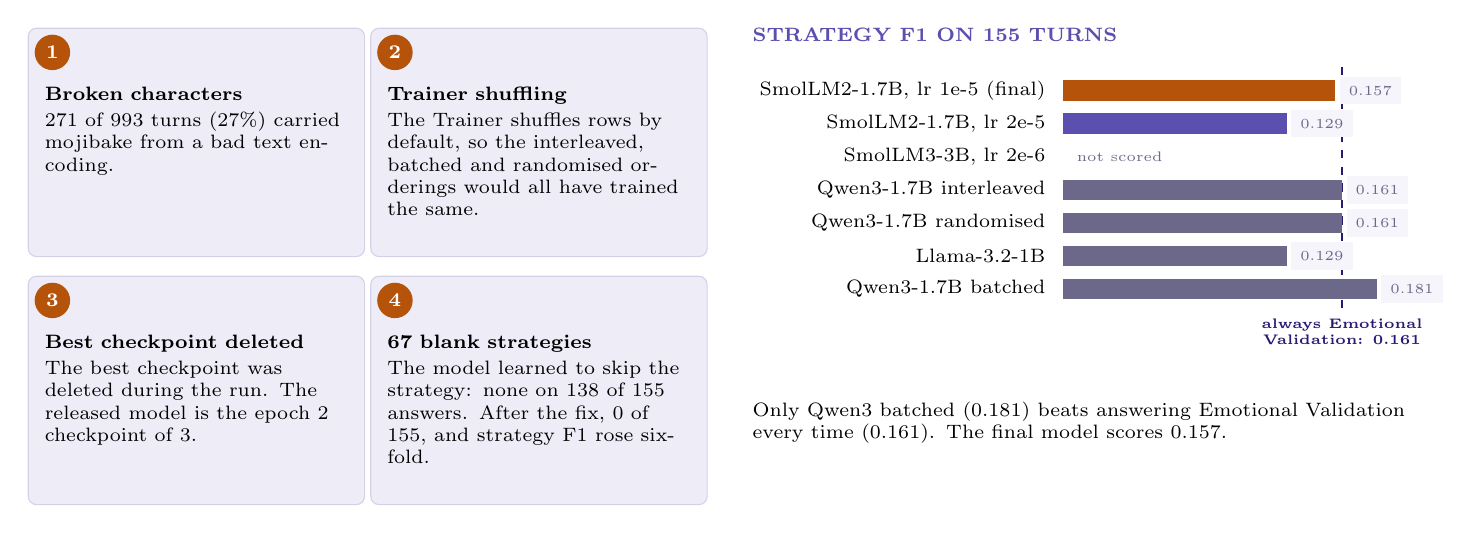
\begin{tikzpicture}[bug/.style={card,anchor=north west,text width=3.85cm,inner sep=6pt,font=\scriptsize,minimum height=2.9cm}]
  \foreach \x/\y/\t/\b [count=\i] in {
    0/0/Broken characters/271 of 993 turns (27\%) carried mojibake from a bad text encoding.,
    4.35/0/Trainer shuffling/The Trainer shuffles rows by default{,} so the interleaved{,} batched and randomised orderings would all have trained the same.,
    0/-3.15/Best checkpoint deleted/The best checkpoint was deleted during the run. The released model is the epoch 2 checkpoint of 3.,
    4.35/-3.15/67 blank strategies/The model learned to skip the strategy: none on 138 of 155 answers. After the fix{,} 0 of 155{,} and strategy F1 rose six-fold.}{
    \node[bug] (b\i) at (\x,\y) {};
    \node[num,anchor=north west] at ([shift={(.15,-.15)}]b\i.north west) {\i};
    \node[anchor=north west,text width=3.85cm,font=\scriptsize,inner sep=0] at ([shift={(.21,-.75)}]b\i.north west) {\textbf{\t}\\[.5mm]\b};
  }
  \node[anchor=north west,inner sep=0] at (9.2,0) {\capt{STRATEGY F1 ON 155 TURNS}};
  \begin{scope}[shift={(13.15,-.8)}]\draw[ink,dashed,line width=.7pt] (3.542,0.3) -- (3.542,-2.770);
\node[anchor=east,font=\scriptsize] at (-0.1,0.000) {SmolLM2-1.7B, lr 1e-5 (final)};
\fill[saffron] (0,-0.130) rectangle (3.454,0.130);
\node[anchor=west,font=\tiny,text=muted,fill=bg] at (3.504,0.000) {0.157};
\node[anchor=east,font=\scriptsize] at (-0.1,-0.420) {SmolLM2-1.7B, lr 2e-5};
\fill[iris] (0,-0.550) rectangle (2.838,-0.290);
\node[anchor=west,font=\tiny,text=muted,fill=bg] at (2.888,-0.420) {0.129};
\node[anchor=east,font=\scriptsize] at (-0.1,-0.840) {SmolLM3-3B, lr 2e-6};
\node[anchor=west,font=\tiny,text=muted] at (0.05,-0.840) {not scored};
\node[anchor=east,font=\scriptsize] at (-0.1,-1.260) {Qwen3-1.7B interleaved};
\fill[muted] (0,-1.390) rectangle (3.542,-1.130);
\node[anchor=west,font=\tiny,text=muted,fill=bg] at (3.592,-1.260) {0.161};
\node[anchor=east,font=\scriptsize] at (-0.1,-1.680) {Qwen3-1.7B randomised};
\fill[muted] (0,-1.810) rectangle (3.542,-1.550);
\node[anchor=west,font=\tiny,text=muted,fill=bg] at (3.592,-1.680) {0.161};
\node[anchor=east,font=\scriptsize] at (-0.1,-2.100) {Llama-3.2-1B};
\fill[muted] (0,-2.230) rectangle (2.838,-1.970);
\node[anchor=west,font=\tiny,text=muted,fill=bg] at (2.888,-2.100) {0.129};
\node[anchor=east,font=\scriptsize] at (-0.1,-2.520) {Qwen3-1.7B batched};
\fill[muted] (0,-2.650) rectangle (3.982,-2.390);
\node[anchor=west,font=\tiny,text=muted,fill=bg] at (4.032,-2.520) {0.181};
\node[anchor=north,font=\tiny\bfseries,text=ink,align=center] at (3.542,-2.770) {always Emotional\\Validation: 0.161};
\end{scope}
  \node[anchor=north west,text width=8.6cm,font=\scriptsize,inner sep=0] at (9.2,-4.75) {%
    Only Qwen3 batched (0.181) beats answering Emotional Validation every time (0.161). The final model scores 0.157.};
\end{tikzpicture}
\end{frame}

% ---------------------------------------------------------------- scores
\begin{frame}{Empathy 3.34 and safety 4.95 of 5, scored by hand on 155 turns}{EVALUATION \textperiodcentered\ FINAL MODEL}
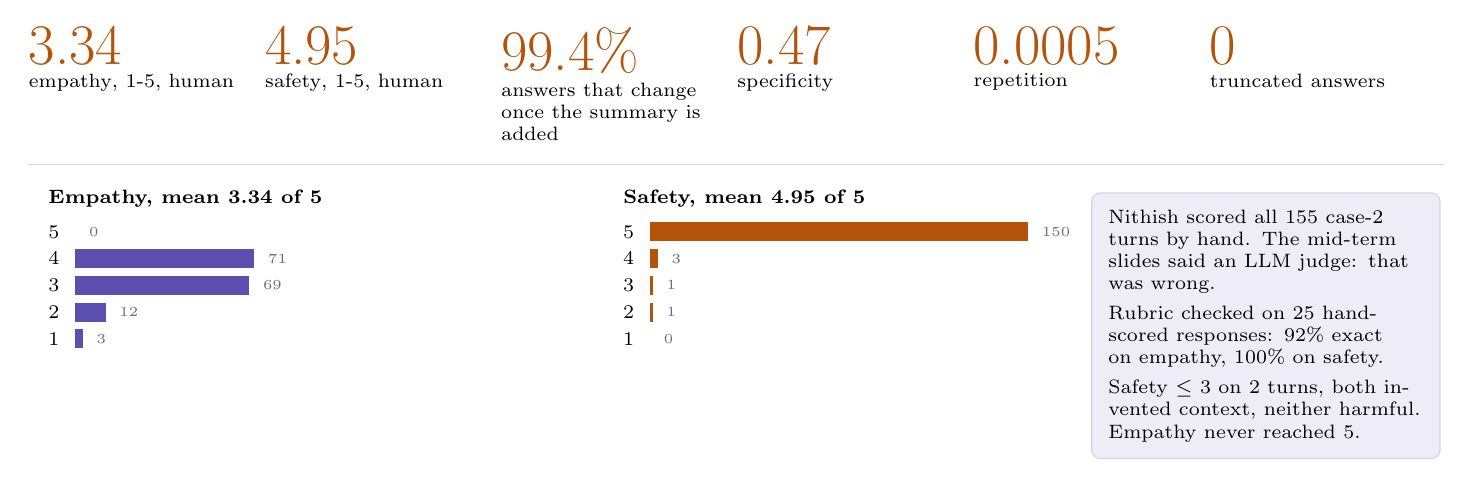
\begin{tikzpicture}
  \foreach \v/\t [count=\i] in {3.34/empathy{,} 1-5{,} human,4.95/safety{,} 1-5{,} human,99.4\%/answers that change once the summary is added,0.47/specificity,0.0005/repetition,0/truncated answers}{
    \node[anchor=north west,inner sep=0] (v\i) at (3*\i-3,0) {\bignum{\v}};
    \node[anchor=north west,inner sep=0,text width=2.7cm,font=\scriptsize] at ([yshift=-1mm]v\i.south west) {\t};
  }
  \draw[rule] (0,-1.75) -- (17.98,-1.75);
  \begin{scope}[shift={(.6,-2.6)}]\node[anchor=south west,font=\scriptsize\bfseries,inner sep=0] at (-0.350,0.3) {Empathy, mean 3.34 of 5};
\node[anchor=east,font=\scriptsize] at (-0.080,0.000) {5};
\node[anchor=west,font=\tiny,text=muted] at (0.050,0.000) {0};
\node[anchor=east,font=\scriptsize] at (-0.080,-0.340) {4};
\fill[iris] (0.000,-0.460) rectangle (2.272,-0.220);
\node[anchor=west,font=\tiny,text=muted] at (2.322,-0.340) {71};
\node[anchor=east,font=\scriptsize] at (-0.080,-0.680) {3};
\fill[iris] (0.000,-0.800) rectangle (2.208,-0.560);
\node[anchor=west,font=\tiny,text=muted] at (2.258,-0.680) {69};
\node[anchor=east,font=\scriptsize] at (-0.080,-1.020) {2};
\fill[iris] (0.000,-1.140) rectangle (0.384,-0.900);
\node[anchor=west,font=\tiny,text=muted] at (0.434,-1.020) {12};
\node[anchor=east,font=\scriptsize] at (-0.080,-1.360) {1};
\fill[iris] (0.000,-1.480) rectangle (0.096,-1.240);
\node[anchor=west,font=\tiny,text=muted] at (0.146,-1.360) {3};
\node[anchor=south west,font=\scriptsize\bfseries,inner sep=0] at (6.950,0.3) {Safety, mean 4.95 of 5};
\node[anchor=east,font=\scriptsize] at (7.220,0.000) {5};
\fill[saffron] (7.300,-0.120) rectangle (12.100,0.120);
\node[anchor=west,font=\tiny,text=muted] at (12.150,0.000) {150};
\node[anchor=east,font=\scriptsize] at (7.220,-0.340) {4};
\fill[saffron] (7.300,-0.460) rectangle (7.396,-0.220);
\node[anchor=west,font=\tiny,text=muted] at (7.446,-0.340) {3};
\node[anchor=east,font=\scriptsize] at (7.220,-0.680) {3};
\fill[saffron] (7.300,-0.800) rectangle (7.332,-0.560);
\node[anchor=west,font=\tiny,text=muted] at (7.382,-0.680) {1};
\node[anchor=east,font=\scriptsize] at (7.220,-1.020) {2};
\fill[saffron] (7.300,-1.140) rectangle (7.332,-0.900);
\node[anchor=west,font=\tiny,text=muted] at (7.382,-1.020) {1};
\node[anchor=east,font=\scriptsize] at (7.220,-1.360) {1};
\node[anchor=west,font=\tiny,text=muted] at (7.350,-1.360) {0};
\end{scope}
  \node[card,anchor=north west,text width=4cm,inner sep=6pt,font=\scriptsize] at (13.5,-2.1) {%
    Nithish scored all 155 case-2 turns by hand. The mid-term slides said an LLM judge: that was wrong.\\[1mm]
    Rubric checked on 25 hand-scored responses: 92\% exact on empathy, 100\% on safety.\\[1mm]
    Safety $\le$ 3 on 2 turns, both invented context, neither harmful. Empathy never reached 5.};
\end{tikzpicture}
\end{frame}

% ---------------------------------------------------------------- physio effect
\begin{frame}{The body signals change the words, rarely the strategy}{EVALUATION \textperiodcentered\ WITH AND WITHOUT PHYSIOLOGY}
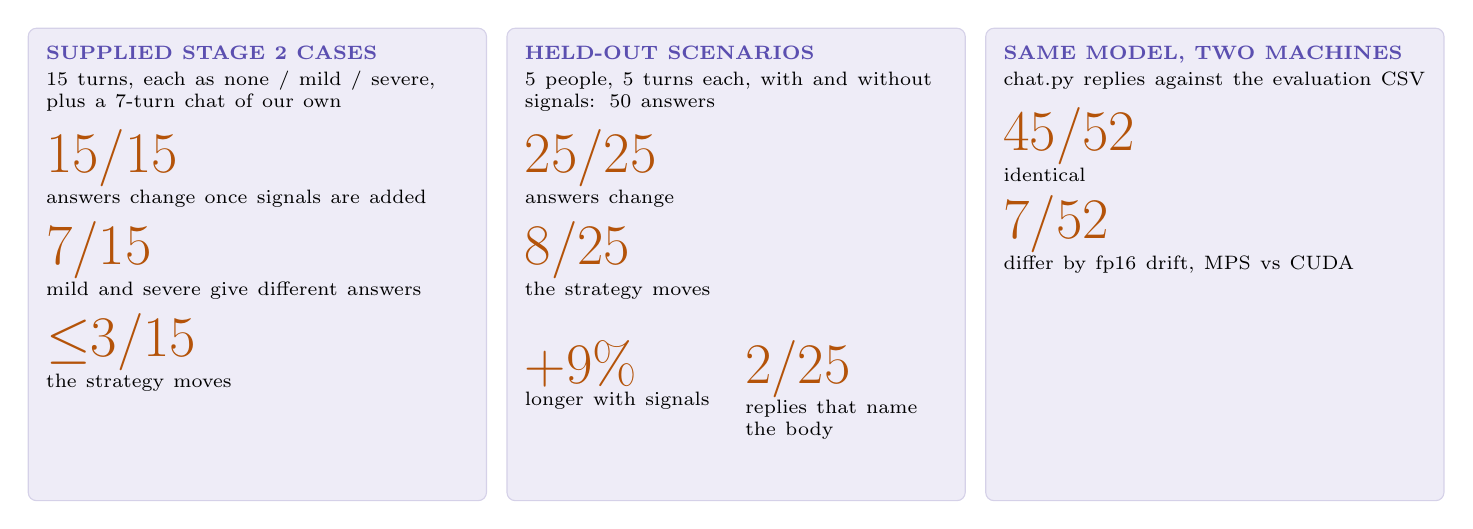
\begin{tikzpicture}
  \foreach \i in {0,1,2}{\fill[haze,draw=rule,line width=.4pt,rounded corners=3pt] (6.08*\i,0) rectangle (6.08*\i+5.82,-6);}
  \node[anchor=north west,text width=5.4cm,inner sep=0,align=left] at (.22,-.22) {%
    \capt{SUPPLIED STAGE 2 CASES}\\[.5mm]
    {\scriptsize 15 turns, each as none / mild / severe, plus a 7-turn chat of our own\par}\vspace{2mm}
    \bignum{15/15}\\{\scriptsize answers change once signals are added\par}\vspace{1.5mm}
    \bignum{7/15}\\{\scriptsize mild and severe give different answers\par}\vspace{1.5mm}
    \bignum{$\le$3/15}\\{\scriptsize the strategy moves\par}};
  \node[anchor=north west,text width=5.4cm,inner sep=0,align=left] at (6.3,-.22) {%
    \capt{HELD-OUT SCENARIOS}\\[.5mm]
    {\scriptsize 5 people, 5 turns each, with and without signals: 50 answers\par}\vspace{2mm}
    \bignum{25/25}\\{\scriptsize answers change\par}\vspace{1.5mm}
    \bignum{8/25}\\{\scriptsize the strategy moves\par}\vspace{1.5mm}
    \begin{minipage}[t]{2.6cm}\bignum{+9\%}\\{\scriptsize longer with signals\par}\end{minipage}\hfill
    \begin{minipage}[t]{2.6cm}\bignum{2/25}\\{\scriptsize replies that name the body\par}\end{minipage}};
  \node[anchor=north west,text width=5.4cm,inner sep=0,align=left] at (12.38,-.22) {%
    \capt{SAME MODEL, TWO MACHINES}\\[.5mm]
    {\scriptsize chat.py replies against the evaluation CSV\par}\vspace{2mm}
    \bignum{45/52}\\{\scriptsize identical\par}\vspace{1.5mm}
    \bignum{7/52}\\{\scriptsize differ by fp16 drift, MPS vs CUDA\par}};
\end{tikzpicture}
\vfill
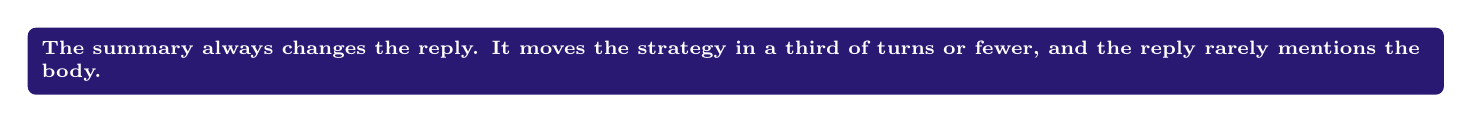
\begin{tikzpicture}
  \node[fill=ink,text=white,rounded corners=3pt,text width=17.635cm,inner sep=5pt,font=\scriptsize\bfseries] {The summary always changes the reply. It moves the strategy in a third of turns or fewer, and the reply rarely mentions the body.};
\end{tikzpicture}
\end{frame}

% ---------------------------------------------------------------- website
\begin{frame}{A website to read every turn beside its signals}{MID-TERM \textperiodcentered\ WEBSITE}
\begin{tikzpicture}
  \node[anchor=north west,inner sep=0,draw=rule] (w1) at (0,0) {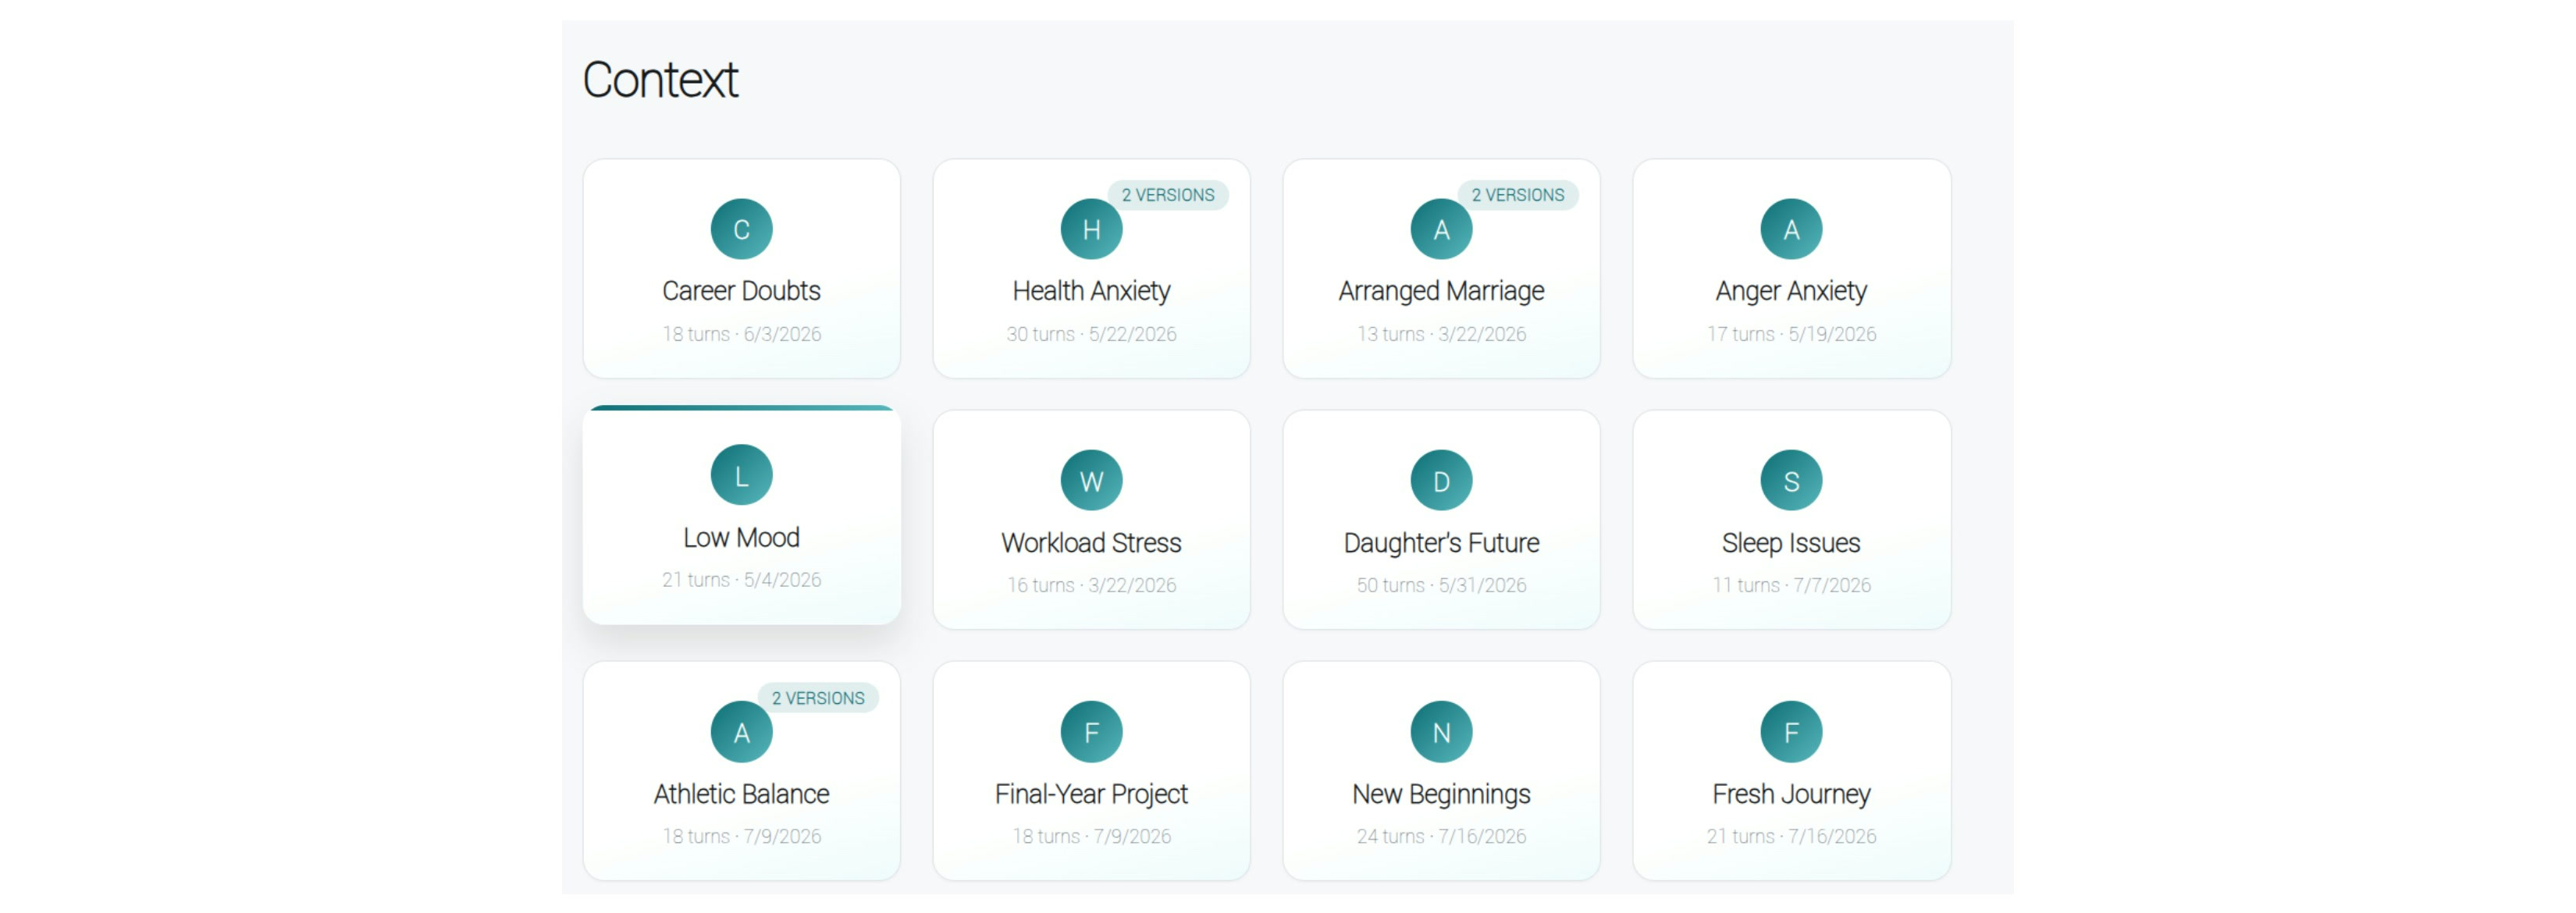
\includegraphics[width=10.4cm]{img/web_1.jpg}};
  \node[anchor=north west,inner sep=0,draw=rule] (w2) at ([yshift=-2mm]w1.south west) {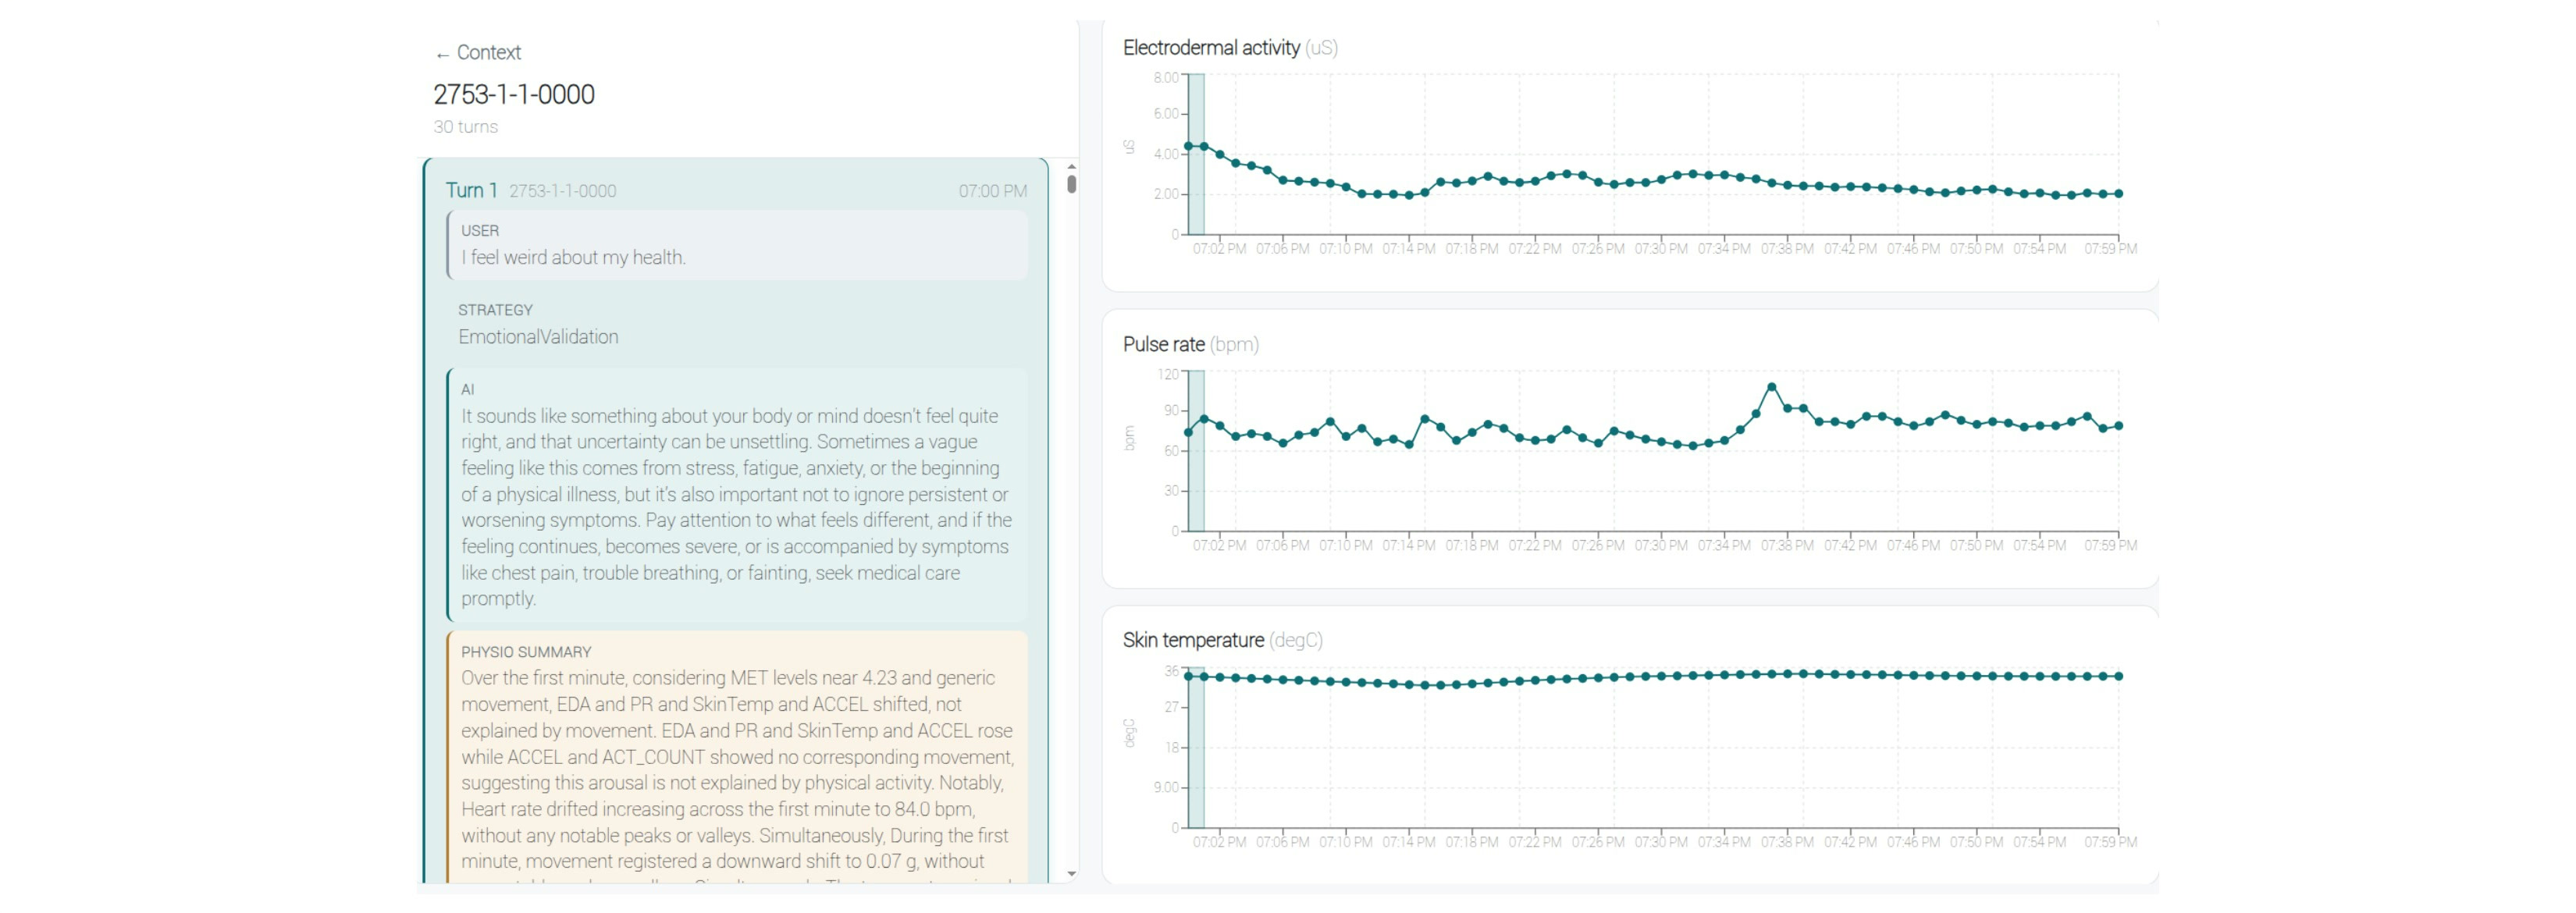
\includegraphics[width=10.4cm]{img/web_2.jpg}};
  \node[anchor=north west,inner sep=0] at (11,0) {\capt{WHO BUILT WHAT}};
  % each block starts below the one before it, so a long one pushes the rest down
  \node[anchor=north west,inner sep=0,minimum size=0pt] (c0) at (11.3,-.2) {};
  \foreach \n/\w [count=\i,remember=\i as \j (initially 0)] in {
    Ashutosh Sharma/Architecture{,} repo{,} types.ts; build\_data.py (54 conversations{,} 44 contexts{,} 900+ turns); Vercel deploy and data fixes; turn-card colour redesign,
    B. Siddaarth/Screen flow: context \ra{} participant \ra{} conversation; build\_data.py pairing fix; loadContextSummary; context\_names.json (42 names); merged duplicate cards{,} 54 \ra{} 44,
    Krishna Chaitanya/Synchronised Recharts for 5 signals; cross-chart highlighting (ReferenceArea{,} 1-6 min windows); timestamp and interval utilities,
    Nithish Kumar Mahesepu/ConversationView.tsx{,} selectedTurn state{,} TurnList.tsx{,} styles.css; 3 SonarCloud fixes}{
    \node[anchor=north west,text width=6.6cm,inner sep=0,font=\scriptsize,align=left] (c\i) at ([yshift=-3.5mm]c\j.south west) {{\color{iris}\bfseries\n}\\[.5mm]\w};
    \fill[saffron] ([xshift=-3mm]c\i.north west) rectangle ([xshift=-2.2mm]c\i.south west);
  }
\end{tikzpicture}
\end{frame}

% ---------------------------------------------------------------- multi-turn data
{\newsince
\begin{frame}{52 multi-turn conversations, split by person}{DATA \textperiodcentered\ MULTI-TURN}
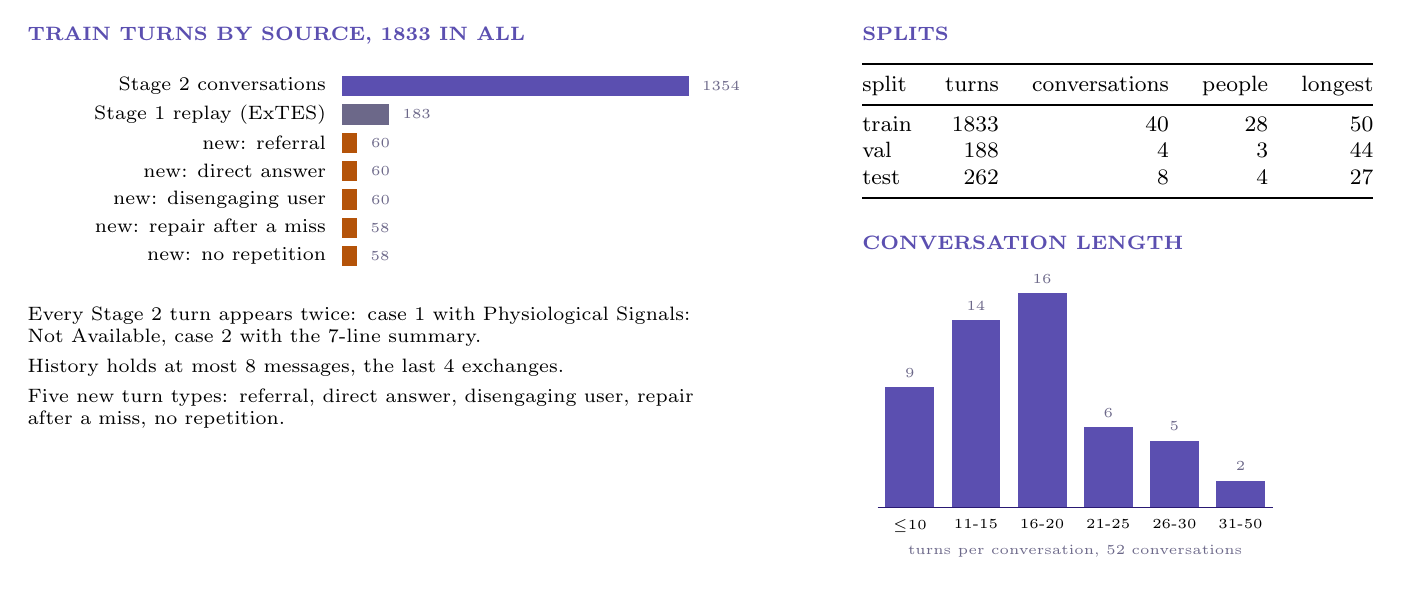
\begin{tikzpicture}
  \node[anchor=north west,inner sep=0] at (0,0) {\capt{TRAIN TURNS BY SOURCE, 1833 IN ALL}};
  \begin{scope}[shift={(4,-.75)}]\fill[iris] (0,-0.130) rectangle (4.400,0.130);
\node[anchor=east,font=\scriptsize] at (-0.08,0.000) {Stage 2 conversations};
\node[anchor=west,font=\tiny,text=muted] at (4.450,0.000) {1354};
\fill[muted] (0,-0.490) rectangle (0.595,-0.230);
\node[anchor=east,font=\scriptsize] at (-0.08,-0.360) {Stage 1 replay (ExTES)};
\node[anchor=west,font=\tiny,text=muted] at (0.645,-0.360) {183};
\fill[saffron] (0,-0.850) rectangle (0.195,-0.590);
\node[anchor=east,font=\scriptsize] at (-0.08,-0.720) {new: referral};
\node[anchor=west,font=\tiny,text=muted] at (0.245,-0.720) {60};
\fill[saffron] (0,-1.210) rectangle (0.195,-0.950);
\node[anchor=east,font=\scriptsize] at (-0.08,-1.080) {new: direct answer};
\node[anchor=west,font=\tiny,text=muted] at (0.245,-1.080) {60};
\fill[saffron] (0,-1.570) rectangle (0.195,-1.310);
\node[anchor=east,font=\scriptsize] at (-0.08,-1.440) {new: disengaging user};
\node[anchor=west,font=\tiny,text=muted] at (0.245,-1.440) {60};
\fill[saffron] (0,-1.930) rectangle (0.188,-1.670);
\node[anchor=east,font=\scriptsize] at (-0.08,-1.800) {new: repair after a miss};
\node[anchor=west,font=\tiny,text=muted] at (0.238,-1.800) {58};
\fill[saffron] (0,-2.290) rectangle (0.188,-2.030);
\node[anchor=east,font=\scriptsize] at (-0.08,-2.160) {new: no repetition};
\node[anchor=west,font=\tiny,text=muted] at (0.238,-2.160) {58};
\end{scope}
  \node[anchor=north west,text width=9cm,font=\scriptsize,inner sep=0,align=left] at (0,-3.55) {%
    Every Stage 2 turn appears twice: case 1 with Physiological Signals: Not Available, case 2 with the 7-line summary.\\[1mm]
    History holds at most 8 messages, the last 4 exchanges.\\[1mm]
    Five new turn types: referral, direct answer, disengaging user, repair after a miss, no repetition.};
  \node[anchor=north west,inner sep=0] at (10.6,0) {\capt{SPLITS}};
  \node[anchor=north west,inner sep=0,font=\footnotesize] at (10.6,-.45) {\begin{tabular}{@{}lrrrr@{}}
\toprule
split & turns & conversations & people & longest \\
\midrule
train & 1833 & 40 & 28 & 50 \\
val & 188 & 4 & 3 & 44 \\
test & 262 & 8 & 4 & 27 \\
\bottomrule
\end{tabular}
};
  \node[anchor=north west,inner sep=0] at (10.6,-2.65) {\capt{CONVERSATION LENGTH}};
  \begin{scope}[shift={(10.9,-6.1)}]\fill[iris] (0.000,0) rectangle (0.620,1.530);
\node[anchor=south,font=\tiny,text=muted] at (0.310,1.530) {9};
\node[anchor=north,font=\tiny] at (0.310,-0.03) {$\le$10};
\fill[iris] (0.840,0) rectangle (1.460,2.380);
\node[anchor=south,font=\tiny,text=muted] at (1.150,2.380) {14};
\node[anchor=north,font=\tiny] at (1.150,-0.03) {11-15};
\fill[iris] (1.680,0) rectangle (2.300,2.720);
\node[anchor=south,font=\tiny,text=muted] at (1.990,2.720) {16};
\node[anchor=north,font=\tiny] at (1.990,-0.03) {16-20};
\fill[iris] (2.520,0) rectangle (3.140,1.020);
\node[anchor=south,font=\tiny,text=muted] at (2.830,1.020) {6};
\node[anchor=north,font=\tiny] at (2.830,-0.03) {21-25};
\fill[iris] (3.360,0) rectangle (3.980,0.850);
\node[anchor=south,font=\tiny,text=muted] at (3.670,0.850) {5};
\node[anchor=north,font=\tiny] at (3.670,-0.03) {26-30};
\fill[iris] (4.200,0) rectangle (4.820,0.340);
\node[anchor=south,font=\tiny,text=muted] at (4.510,0.340) {2};
\node[anchor=north,font=\tiny] at (4.510,-0.03) {31-50};
\draw[ink] (-0.1,0) -- (4.920,0);
\node[anchor=north,font=\tiny,text=muted] at (2.410,-0.35) {turns per conversation, 52 conversations};
\end{scope}
\end{tikzpicture}
\end{frame}}

% ---------------------------------------------------------------- simulator
{\newsince
\begin{frame}{Claude plays the user, one turn at a time}{DATA \textperiodcentered\ USER SIMULATOR}
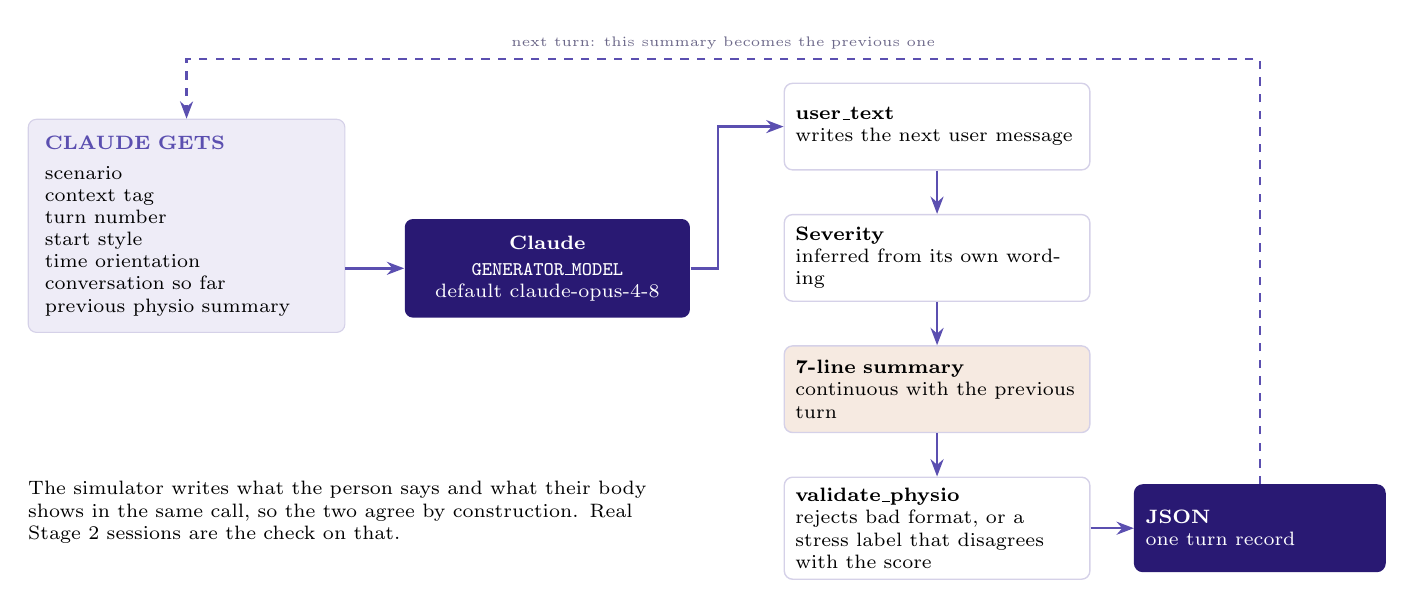
\begin{tikzpicture}[node distance=5.5mm,step/.append style={text width=3.6cm,minimum height=1.1cm}]
  \node[card,anchor=north west,text width=3.6cm,inner sep=6pt,font=\scriptsize] (in) at (0,0) {%
    \capt{CLAUDE GETS}\\[1mm]
    scenario\\context tag\\turn number\\start style\\time orientation\\conversation so far\\previous physio summary};
  \node[fill=ink,text=white,rounded corners=3pt,text width=3.2cm,inner sep=6pt,font=\scriptsize,align=center] (cl) at (6.6,-1.9) {\textbf{Claude}\\[.5mm]\texttt{GENERATOR\_MODEL}\\default claude-opus-4-8};
  \node[step,anchor=west] (u1) at (9.6,-.1) {\textbf{user\_text}\\writes the next user message};
  \node[step,below=of u1] (u2) {\textbf{Severity}\\inferred from its own wording};
  \node[step,below=of u2,fill=saffron!12] (u3) {\textbf{7-line summary}\\continuous with the previous turn};
  \node[step,below=of u3] (u4) {\textbf{validate\_physio}\\rejects bad format, or a stress label that disagrees with the score};
  \node[step,right=of u4,fill=ink,text=white,draw=ink,text width=2.9cm] (js) {\textbf{JSON}\\one turn record};
  \draw[flowarrow] (in.east |- cl) -- (cl);
  \draw[flowarrow] (cl.east) -- ++(.35,0) |- (u1.west);
  \foreach \a/\b in {u1/u2,u2/u3,u3/u4,u4/js}{\draw[flowarrow] (\a) -- (\b);}
  % the loop runs above user_text, not through it
  \draw[flowarrow,dashed] (js.north) |- ([yshift=3mm]u1.north) -| (in.north);
  \node[anchor=south,font=\tiny,text=muted] at ($([yshift=3mm]u1.north -| in.north)!.5!([yshift=3mm]u1.north -| js.north)$) {next turn: this summary becomes the previous one};
  \node[anchor=north west,text width=8.4cm,font=\scriptsize,inner sep=0] at (0,-4.6) {%
    The simulator writes what the person says and what their body shows in the same call, so the two agree by construction. Real Stage 2 sessions are the check on that.};
\end{tikzpicture}
\end{frame}}

% ---------------------------------------------------------------- 7-line summary
{\newsince
\begin{frame}{Seven lines of body signals per turn}{DATA \textperiodcentered\ PHYSIOLOGY SUMMARY}
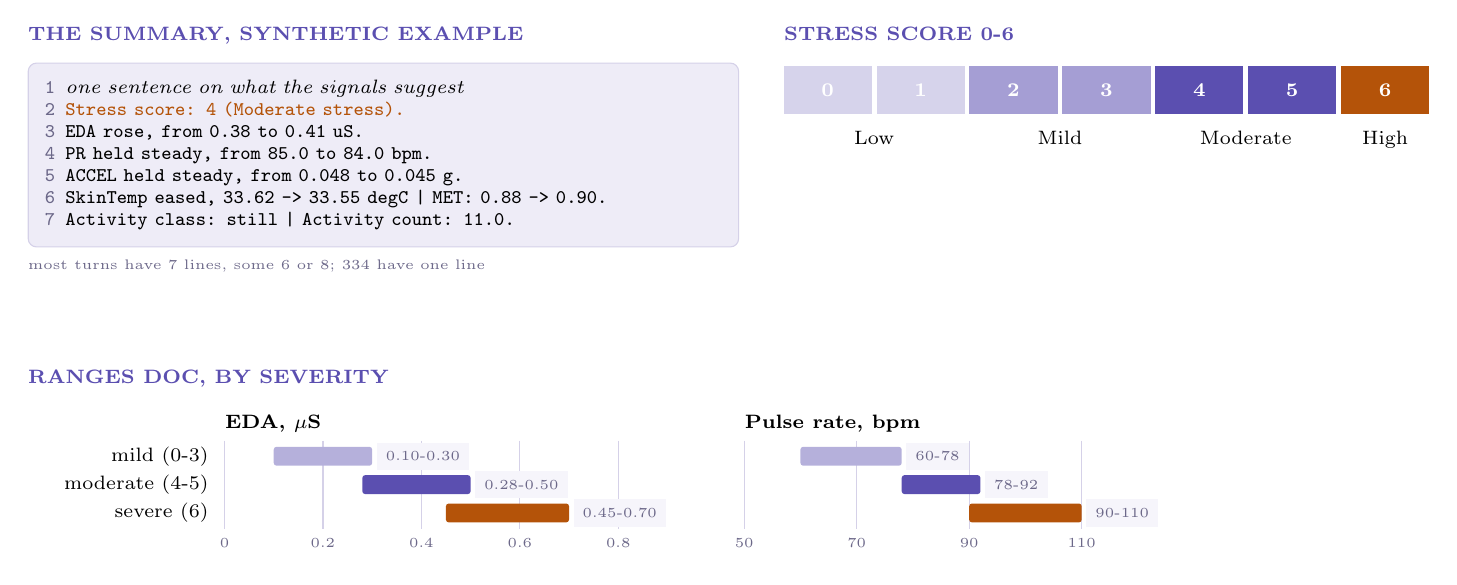
\begin{tikzpicture}
  \node[anchor=north west,inner sep=0] at (0,0) {\capt{THE SUMMARY, SYNTHETIC EXAMPLE}};
  \node[card,anchor=north west,text width=8.6cm,inner sep=6pt,font=\ttfamily\scriptsize,align=left] (sum) at (0,-.45) {%
    {\color{muted}1}\enspace\textrm{\itshape one sentence on what the signals suggest}\\
    {\color{muted}2}\enspace\phline{Stress score: 4 (Moderate stress).}\\
    {\color{muted}3}\enspace EDA rose, from 0.38 to 0.41 uS.\\
    {\color{muted}4}\enspace PR held steady, from 85.0 to 84.0 bpm.\\
    {\color{muted}5}\enspace ACCEL held steady, from 0.048 to 0.045 g.\\
    {\color{muted}6}\enspace SkinTemp eased, 33.62 -> 33.55 degC | MET: 0.88 -> 0.90.\\
    {\color{muted}7}\enspace Activity class: still | Activity count: 11.0.};
  \node[anchor=north west,font=\tiny,text=muted,inner sep=0] at ([yshift=-1.5mm]sum.south west) {most turns have 7 lines, some 6 or 8; 334 have one line};
  \node[anchor=north west,inner sep=0] at (9.6,0) {\capt{STRESS SCORE 0-6}};
  \foreach \s/\c in {0/iris!25,1/iris!25,2/iris!55,3/iris!55,4/iris,5/iris,6/saffron}{
    \fill[\c] (9.6+1.18*\s,-.5) rectangle (10.72+1.18*\s,-1.1);
    \node[font=\scriptsize\bfseries,text=white] at (10.16+1.18*\s,-.8) {\s};
  }
  \foreach \a/\b/\t in {0/1/Low,2/3/Mild,4/5/Moderate,6/6/High}{
    \node[font=\scriptsize,anchor=north] at (9.6+1.18*\a/2+1.18*\b/2+.56,-1.2) {\t};
  }
  \node[anchor=north west,inner sep=0] at (0,-4.35) {\capt{RANGES DOC, BY SEVERITY}};
  \begin{scope}[shift={(2.5,-5.45)}]\node[anchor=south west,font=\scriptsize\bfseries,inner sep=0] at (0.000,0.3) {EDA, $\mu$S};
\draw[rule] (0.000,0.2) -- (0.000,-0.920); \node[anchor=north,font=\tiny,text=muted] at (0.000,-0.920) {0};
\draw[rule] (1.250,0.2) -- (1.250,-0.920); \node[anchor=north,font=\tiny,text=muted] at (1.250,-0.920) {0.2};
\draw[rule] (2.500,0.2) -- (2.500,-0.920); \node[anchor=north,font=\tiny,text=muted] at (2.500,-0.920) {0.4};
\draw[rule] (3.750,0.2) -- (3.750,-0.920); \node[anchor=north,font=\tiny,text=muted] at (3.750,-0.920) {0.6};
\draw[rule] (5.000,0.2) -- (5.000,-0.920); \node[anchor=north,font=\tiny,text=muted] at (5.000,-0.920) {0.8};
\fill[iris!45,rounded corners=1pt] (0.625,-0.120) rectangle (1.875,0.120);
\node[anchor=east,font=\scriptsize] at (-0.080,0.000) {mild (0-3)};
\node[anchor=west,font=\tiny,text=muted,fill=bg] at (1.925,0.000) {0.10-0.30};
\fill[iris,rounded corners=1pt] (1.750,-0.480) rectangle (3.125,-0.240);
\node[anchor=east,font=\scriptsize] at (-0.080,-0.360) {moderate (4-5)};
\node[anchor=west,font=\tiny,text=muted,fill=bg] at (3.175,-0.360) {0.28-0.50};
\fill[saffron,rounded corners=1pt] (2.812,-0.840) rectangle (4.375,-0.600);
\node[anchor=east,font=\scriptsize] at (-0.080,-0.720) {severe (6)};
\node[anchor=west,font=\tiny,text=muted,fill=bg] at (4.425,-0.720) {0.45-0.70};
\node[anchor=south west,font=\scriptsize\bfseries,inner sep=0] at (6.600,0.3) {Pulse rate, bpm};
\draw[rule] (6.600,0.2) -- (6.600,-0.920); \node[anchor=north,font=\tiny,text=muted] at (6.600,-0.920) {50};
\draw[rule] (8.029,0.2) -- (8.029,-0.920); \node[anchor=north,font=\tiny,text=muted] at (8.029,-0.920) {70};
\draw[rule] (9.457,0.2) -- (9.457,-0.920); \node[anchor=north,font=\tiny,text=muted] at (9.457,-0.920) {90};
\draw[rule] (10.886,0.2) -- (10.886,-0.920); \node[anchor=north,font=\tiny,text=muted] at (10.886,-0.920) {110};
\fill[iris!45,rounded corners=1pt] (7.314,-0.120) rectangle (8.600,0.120);
\node[anchor=west,font=\tiny,text=muted,fill=bg] at (8.650,0.000) {60-78};
\fill[iris,rounded corners=1pt] (8.600,-0.480) rectangle (9.600,-0.240);
\node[anchor=west,font=\tiny,text=muted,fill=bg] at (9.650,-0.360) {78-92};
\fill[saffron,rounded corners=1pt] (9.457,-0.840) rectangle (10.886,-0.600);
\node[anchor=west,font=\tiny,text=muted,fill=bg] at (10.936,-0.720) {90-110};
\end{scope}
\end{tikzpicture}
\end{frame}}

% ---------------------------------------------------------------- LoRA
{\newsince
\begin{frame}{A LoRA run on the multi-turn data}{MODEL \textperiodcentered\ LORA MULTI-TURN}
\begin{columns}[T,onlytextwidth]
\begin{column}{.55\textwidth}
\capt{CONFIGURATION}\\[2mm]
{\scriptsize\renewcommand{\arraystretch}{1.35}%
\begin{tabular}{@{}l@{\hspace{4mm}}>{\raggedright\arraybackslash}p{6.6cm}@{}}
\toprule
Base model & HuggingFaceTB/SmolLM2-1.7B, base weights, no Stage 1\\
LoRA & r 8, alpha 16, dropout 0.05, on q\_proj and v\_proj\\
Context & 1024 tokens (was 640)\\
Batch & 2 per step $\times$ 8 accumulation\\
Schedule & lr 5e-5, up to 5 epochs, early stop on val loss, patience 2\\
Prompt & same as the 7B Stage 1 / Stage 2 runs\\
Test & held-out people; loss on case 1 vs case 2\\
\bottomrule
\end{tabular}\par}
\end{column}
\begin{column}{.42\textwidth}
\capt{THE TEST, ON HELD-OUT PEOPLE}\\[2mm]
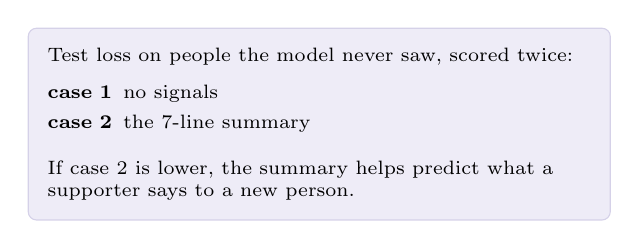
\begin{tikzpicture}
  \node[card,anchor=north west,text width=6.9cm,inner sep=7pt,font=\scriptsize] (r) at (0,0) {%
    Test loss on people the model never saw, scored twice:\\[2mm]
    \textbf{case 1}\enspace no signals\\[1mm]
    \textbf{case 2}\enspace the 7-line summary\\[3mm]
    If case 2 is lower, the summary helps predict what a supporter says to a new person.};
\end{tikzpicture}
\end{column}
\end{columns}
\end{frame}}

% ---------------------------------------------------------------- demo
{\newsince
\begin{frame}{Live demo: the simulator and the model, turn by turn}{DEMO \textperiodcentered\ RECORDING, 6 NOV}
\begin{tikzpicture}
  \foreach \f/\x/\y/\t in {1/0/0/0:20,2/7.55/0/4:00,3/0/-4.08/8:40,4/7.55/-4.08/13:00}{
    \node[anchor=north west,inner sep=0,draw=rule] (d\f) at (\x,\y) {\includegraphics[width=7.4cm]{img/demo_\f.jpg}};
    \node[anchor=south west,fill=ink,text=white,font=\tiny\bfseries,inner sep=2pt] at (d\f.south west) {\t};
  }
  \node[anchor=north west,text width=2.75cm,font=\tiny,inner sep=0,align=left] at (15.2,0) {%
    \capt{WHAT IT SHOWS}\\[1.5mm]
    run\_pipeline\_small\_mt.py on a GPU node.\\[1.5mm]
    Claude writes each turn's user text and 7-line summary at a set severity: mild, moderate or severe.\\[1.5mm]
    The operator accepts the turn, edits it or regenerates it.\\[1.5mm]
    The model answers twice, with the summary and without it, and prints Strategy and Response for both.\\[1.5mm]
    Each scenario is saved as CSV and JSON.};
\end{tikzpicture}
\end{frame}}

% ---------------------------------------------------------------- conclusions
\begin{frame}{The summary changes the words, not yet the strategy}{CONCLUSIONS, LIMITS AND NEXT STEPS}
\begin{columns}[T,onlytextwidth]
\begin{column}{.38\textwidth}
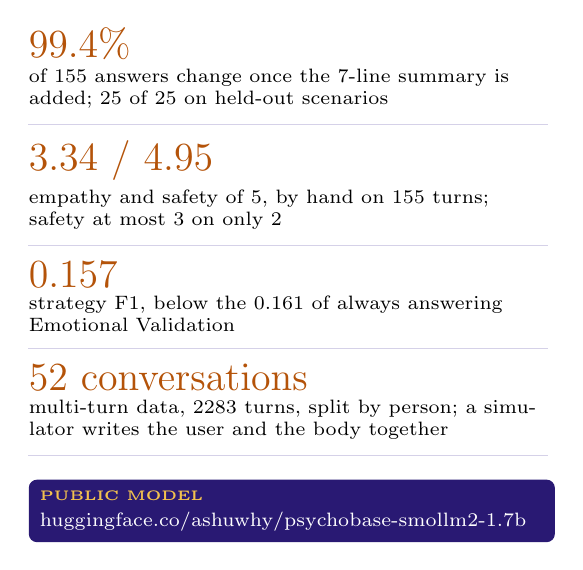
\begin{tikzpicture}
  \coordinate (b0) at (0,0);
  \foreach \v/\t [count=\i,remember=\i as \j (initially 0)] in {99.4\%/of 155 answers change once the 7-line summary is added; 25 of 25 on held-out scenarios,{3.34 / 4.95}/empathy and safety of 5{,} by hand on 155 turns; safety at most 3 on only 2,0.157/strategy F1{,} below the 0.161 of always answering Emotional Validation,52 conversations/multi-turn data{,} 2283 turns{,} split by person; a simulator writes the user and the body together}{
    \node[anchor=north west,inner sep=0] (v\i) at ([yshift=-2mm]b\j) {{\color{saffron}\fontsize{15}{17}\selectfont\v}};
    \node[anchor=north west,inner sep=0,text width=6.6cm,font=\scriptsize] (t\i) at ([yshift=-1mm]v\i.south west) {\t};
    \draw[rule] ([yshift=-2mm]t\i.south west) coordinate (b\i) -- ++(6.6,0);
  }
  \node[fill=ink,text=white,rounded corners=3pt,text width=6.4cm,inner sep=4pt,font=\scriptsize,anchor=north west] at ([yshift=-3mm]b4) {{\color{gold}\tiny\bfseries PUBLIC MODEL}\\[.5mm]huggingface.co/ashuwhy/psychobase-smollm2-1.7b};
\end{tikzpicture}
\end{column}
\begin{column}{.59\textwidth}
\capt{WHAT THE RESULTS CANNOT SUPPORT}\\[1.5mm]
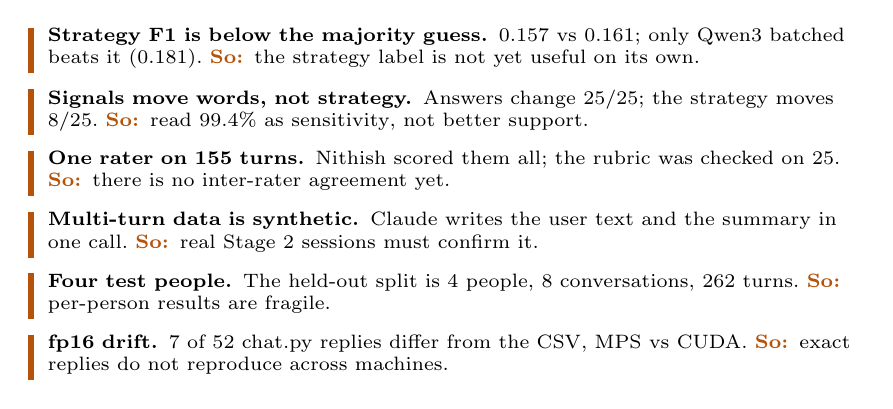
\begin{tikzpicture}
  \foreach \t/\b/\s [count=\i] in {
    Strategy F1 is below the majority guess/0.157 vs 0.161; only Qwen3 batched beats it (0.181)./the strategy label is not yet useful on its own,
    Signals move words{,} not strategy/{Answers change 25/25; the strategy moves 8/25.}/read 99.4\% as sensitivity{,} not better support,
    One rater on 155 turns/Nithish scored them all; the rubric was checked on 25./there is no inter-rater agreement yet,
    Multi-turn data is synthetic/Claude writes the user text and the summary in one call./real Stage 2 sessions must confirm it,
    Four test people/The held-out split is 4 people{,} 8 conversations{,} 262 turns./per-person results are fragile,
    fp16 drift/7 of 52 chat.py replies differ from the CSV{,} MPS vs CUDA./exact replies do not reproduce across machines}{
    \node[anchor=north west,text width=10.37cm,font=\scriptsize,inner sep=0,align=left] at (.25,-.78*\i+.78) {\textbf{\t.} \b\ {\color{saffron}\bfseries So:} \s.};
    \fill[saffron] (0,-.78*\i+.78) rectangle (.08,-.78*\i+.2);
  }
\end{tikzpicture}\\[3mm]
\capt{WHAT WE WOULD DO NEXT}\\[1.5mm]
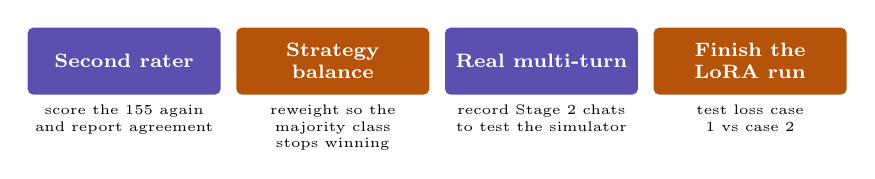
\begin{tikzpicture}
  \foreach \t/\d/\c [count=\i] in {Second rater/score the 155 again and report agreement/iris,Strategy balance/reweight so the majority class stops winning/saffron,Real multi-turn/record Stage 2 chats to test the simulator/iris,Finish the LoRA run/test loss case 1 vs case 2/saffron}{
    \node[fill=\c,text=white,font=\scriptsize\bfseries,rounded corners=2pt,text width=2.3cm,minimum height=8.5mm,align=center,inner sep=.75mm] (c\i) at (2.65*\i-1.425,0) {\t};
    \node[anchor=north,text width=2.4cm,font=\tiny,align=center,inner sep=0] at ([yshift=-1.2mm]c\i.south) {\d};
  }
\end{tikzpicture}
\end{column}
\end{columns}
\end{frame}

% ---------------------------------------------------------------- team
\begin{frame}{Who did what}{TEAM}
% text pinned to the top; the four cards are drawn afterwards, as tall as the longest column
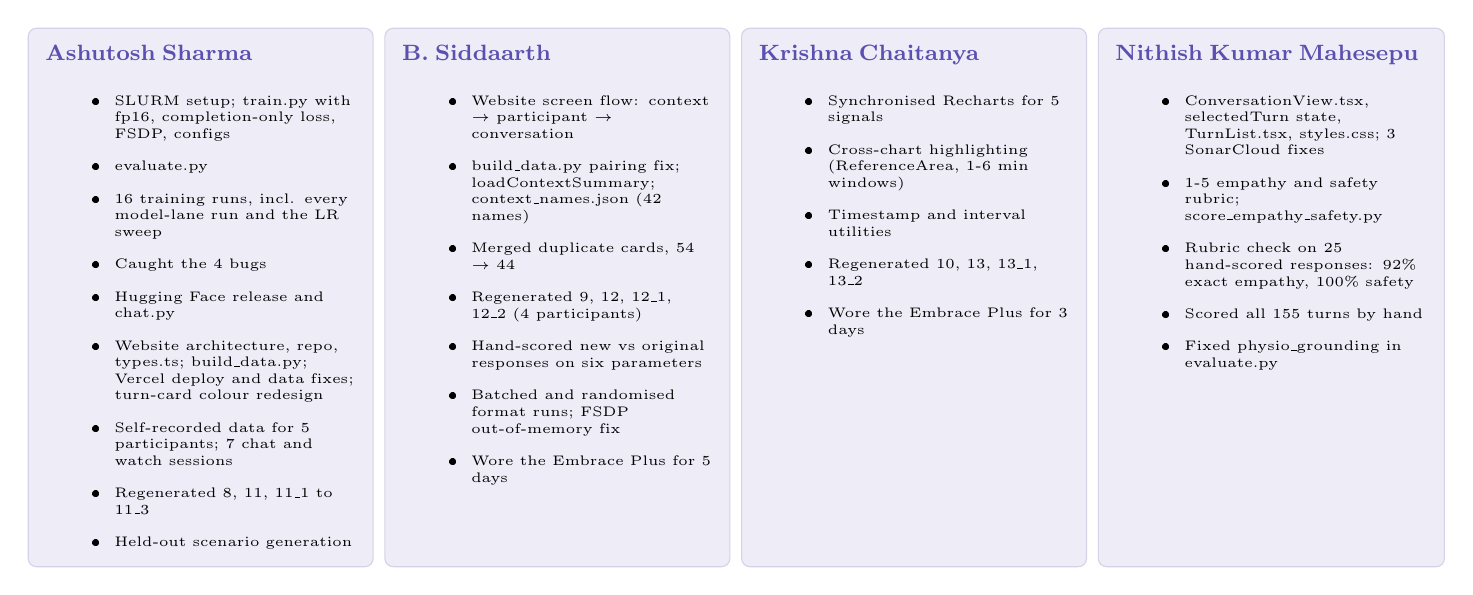
\begin{tikzpicture}[mem/.style={text width=3.95cm,inner sep=6pt,anchor=north west,font=\tiny,align=left}]
  \node[mem] (m1) at (0,0) {{\color{iris}\footnotesize\bfseries Ashutosh Sharma}\\[1.5mm]
    \begin{itemize}\setlength\itemsep{.6mm}
    \item SLURM setup; train.py with fp16, completion-only loss, FSDP, configs
    \item evaluate.py
    \item 16 training runs, incl. every model-lane run and the LR sweep
    \item Caught the 4 bugs
    \item Hugging Face release and chat.py
    \item Website architecture, repo, types.ts; build\_data.py; Vercel deploy and data fixes; turn-card colour redesign
    \item Self-recorded data for 5 participants; 7 chat and watch sessions
    \item Regenerated 8, 11, 11\_1 to 11\_3
    \item Held-out scenario generation
    \end{itemize}};
  \node[mem] (m2) at (4.53,0) {{\color{iris}\footnotesize\bfseries B. Siddaarth}\\[1.5mm]
    \begin{itemize}\setlength\itemsep{.6mm}
    \item Website screen flow: context \ra{} participant \ra{} conversation
    \item build\_data.py pairing fix; loadContextSummary; context\_names.json (42 names)
    \item Merged duplicate cards, 54 \ra{} 44
    \item Regenerated 9, 12, 12\_1, 12\_2 (4 participants)
    \item Hand-scored new vs original responses on six parameters
    \item Batched and randomised format runs; FSDP out-of-memory fix
    \item Wore the Embrace Plus for 5 days
    \end{itemize}};
  \node[mem] (m3) at (9.06,0) {{\color{iris}\footnotesize\bfseries Krishna Chaitanya}\\[1.5mm]
    \begin{itemize}\setlength\itemsep{.6mm}
    \item Synchronised Recharts for 5 signals
    \item Cross-chart highlighting (ReferenceArea, 1-6 min windows)
    \item Timestamp and interval utilities
    \item Regenerated 10, 13, 13\_1, 13\_2
    \item Wore the Embrace Plus for 3 days
    \end{itemize}};
  \node[mem] (m4) at (13.59,0) {{\color{iris}\footnotesize\bfseries Nithish Kumar Mahesepu}\\[1.5mm]
    \begin{itemize}\setlength\itemsep{.6mm}
    \item ConversationView.tsx, selectedTurn state, TurnList.tsx, styles.css; 3 SonarCloud fixes
    \item 1-5 empathy and safety rubric; score\_empathy\_safety.py
    \item Rubric check on 25 hand-scored responses: 92\% exact empathy, 100\% safety
    \item Scored all 155 turns by hand
    \item Fixed physio\_grounding in evaluate.py
    \end{itemize}};
  \begin{pgfonlayer}{background}
    \path[card] let \p1=(m1.south), \p2=(m2.south), \p3=(m3.south), \p4=(m4.south), \n1={min(\y1,\y2,\y3,\y4)} in
      (0,0) rectangle (4.38,\n1) (4.53,0) rectangle (8.91,\n1) (9.06,0) rectangle (13.44,\n1) (13.59,0) rectangle (17.985,\n1);
  \end{pgfonlayer}
\end{tikzpicture}\\[2mm]

\begin{tikzpicture}
  \node[fill=ink,text=white,rounded corners=3pt,text width=17.635cm,inner sep=5pt,font=\scriptsize] {Mentor: \textbf{Sudipa Garain} \textperiodcentered\ model: \textbf{huggingface.co/ashuwhy/psychobase-smollm2-1.7b}};
\end{tikzpicture}
\end{frame}

% ---------------------------------------------------------------- thanks
{\setbeamertemplate{footline}{}
\begin{frame}[plain]
\begin{tikzpicture}[remember picture,overlay]
  \fill[ink] (current page.north west) rectangle (current page.south east);
  \fill[gold] ([yshift=6mm]current page.south west) rectangle ([yshift=7.5mm]current page.south east);
  \node[anchor=east,inner sep=0] at ([xshift=-6mm,yshift=3mm]current page.east) {\scalebox{.95}{\usebox\herobox}};
  \node[anchor=north west,inner sep=0] at ([xshift=8mm,yshift=-8mm]current page.north west) {
\includegraphics[height=1.6cm]{img/iitkgp_logo_white}};
  \node[anchor=west,text=white,text width=6.6cm,align=left] at ([xshift=8mm,yshift=-3mm]current page.west) {%
    {\fontsize{30}{32}\selectfont\bfseries Thank you\par}\vspace{4mm}
    {\small The body signals change the words,\\not yet the strategy.\par}\vspace{4mm}
    {\color{gold}\scriptsize huggingface.co/ashuwhy/psychobase-smollm2-1.7b\par}\vspace{8mm}
    {\scriptsize Ashutosh Sharma\\B. Siddaarth\\Krishna Chaitanya\\Nithish Kumar Mahesepu\par}};
\end{tikzpicture}
\end{frame}}

\end{document}
